\documentclass[12pt,a4paper]{ctexart}

\usepackage[UTF8]{ctex}
\usepackage{geometry}
\usepackage{graphicx}
\usepackage{enumitem}
\usepackage{hyperref}
\usepackage{listings}
\usepackage{xcolor}
\usepackage{booktabs}
\usepackage{tabularx}
\usepackage{caption}
\usepackage{titlesec}
\usepackage{float}
\usepackage{fancyhdr}
\usepackage{subcaption}

\geometry{left=2.5cm,right=2.5cm,top=2.5cm,bottom=2.5cm}

\pagestyle{fancy}           % 启用 fancyhdr 的页面样式
\fancyhf{}                  % 清空所有页眉和页脚

\fancyfoot[C]{\thepage}     % 页码放在页脚中央（C = Center）
% 或者 \fancyfoot[R]{\thepage}  放在右侧
% 或者 \fancyfoot[L]{\thepage}  放在左侧

\renewcommand{\headrulewidth}{0pt}   % 去掉页眉横线（可选）

\graphicspath{{screenshots/}}

% \hypersetup{
%     colorlinks=true,
%     linkcolor=blue,
%     urlcolor=blue
% }

\ctexset{
    section = {
        format = \centering\bfseries\zihao{-2},
        name = {第, 章}
    }
}

\lstset{
    basicstyle=\ttfamily\small,
    keywordstyle=\color{blue},
    commentstyle=\color{green!60!black},
    numbers=left,
    numberstyle=\tiny,
    frame=single,
    breaklines=true,
    backgroundcolor=\color{gray!5}
}

\title{\textbf{塔防游戏设计文档 \\ \large Tower Defense Game Design Document}}
\author{基于 SFML 2.6 引擎}
\date{\today}

\begin{document}

% \maketitle
\clearpage
\newpage
\pagestyle{empty}
\tableofcontents 
% {\small
% \tableofcontents
% }
\thispagestyle{empty}
\clearpage
\newpage
\pagenumbering{arabic}
\pagestyle{fancy}
\section{概述}

\subsection{游戏简介}

《Tower Defense》是一款基于 SFML 2.6 引擎开发的 2D 塔防游戏。玩家通过在地图上的指定位置建造箭塔、炮塔和冰塔，抵御沿路径前进的敌人波次。游戏包含完整的战役模式、自定义模式、角色系统、商店升级、地图编辑器和作弊码系统。

\subsection{技术栈}

\begin{itemize}
    \item \textbf{编程语言}: C++17
    \item \textbf{图形引擎}: SFML 2.6（system / window / graphics / audio）
    \item \textbf{构建工具}: CMake 3.16+
    \item \textbf{操作系统}: Windows（基于 SFML DLL）
    \item \textbf{资源格式}: JSON（语言文件）、PNG（纹理）、MP3（音频）、TXT（地图数据）
    \item \textbf{项目结构}: include/（头文件）、src/（源码）、assets/（资源文件）
\end{itemize}

\subsection{窗口与网格}

\begin{itemize}
    \item 窗口分辨率: 1024 × 768 像素（固定）
    \item 地图网格: 16 列 × 12 行
    \item 瓦片大小: 64 × 64 像素
    \item 游戏区域: 1024 × 768 像素，UI 覆盖在上层
\end{itemize}

\section{研究目的与意义}

\subsection{研究目的}

本游戏是计算机图形学课程的实践项目，旨在通过开发一个完整的 2D 塔防游戏，深入理解和应用计算机图形学的基本概念与 SFML 游戏引擎的开发流程。具体目的包括：

\begin{enumerate}
    \item 掌握基于瓦片地图（Tile Map）的 2D 场景构建方法
    \item 理解精灵（Sprite）渲染、纹理加载与动画系统的工作原理
    \item 实践游戏循环（Game Loop）、事件处理、碰撞检测等核心图形编程技术
    \item 学习 C++ 面向对象设计在游戏开发中的实际应用（类继承、多态、智能指针）
    \item 探索多语言 UI、存档序列化、地图编辑器等扩展功能的实现方法
\end{enumerate}

\subsection{研究意义}

塔防游戏作为策略类游戏的重要分支，具有规则清晰、系统完整、适合作为图形学教学案例的特点。通过本项目的开发实践：

\begin{itemize}
    \item \textbf{图形学理论验证}：将计算机图形学中的坐标变换、纹理映射、帧动画、碰撞检测等理论应用到实际项目中，加深对理论的理解
    \item \textbf{工程能力培养}：从零搭建完整的游戏工程，涵盖 CMake 构建配置、资源管理、跨平台兼容等工业级实践
    \item \textbf{游戏系统设计}：实践有限状态机（FSM）、组件化设计、数据驱动开发等游戏架构思想
    \item \textbf{交互设计探索}：研究 RTS 风格右键交互、弹出菜单系统、HUD 信息反馈等用户交互模式
    \item \textbf{扩展性验证}：通过战役/自定义双模式、内置地图编辑器、作弊码系统等功能验证游戏框架的扩展能力
\end{itemize}

\section{游戏状态机}

游戏使用有限状态机（FSM）管理不同屏幕，主循环集中在 \texttt{Game::run()} 中。

\begin{figure}[H]
    \centering
    \begin{tabular}{|c|l|c|l|}
        \hline
        \textbf{状态} & \textbf{描述} & \textbf{状态} & \textbf{描述} \\
        \hline
        CharSelect   & 角色选择界面  &  CustomSetup  & 自定义模式参数设置 \\
        CharCreate   & 创建新角色  & Shop         & 商店升级 \\
        CharLoad     & 加载已有角色  & MapEditor    & 地图编辑器 \\
        Menu         & 主菜单  &  Playing      & 游戏进行中 \\
        Settings     & 设置界面  & GameOver     & 游戏失败（生命归零） \\
        CampaignSelect & 战役选关  & GameWon      & 关卡胜利 \\
        \hline
    \end{tabular}
    \caption{游戏状态机各状态}
\end{figure}

\subsection{状态转换流程}

\begin{enumerate}
    \item 启动 → \texttt{CharSelect} → 选择或创建角色
    \item 角色确认 → \texttt{Menu}（主菜单）
    \item 主菜单 → \texttt{CampaignSelect} / \texttt{CustomSetup} / \texttt{Shop} / \texttt{MapEditor} / \texttt{Settings}
    \item 关卡确认 → \texttt{Playing}（开始游戏）
    \item Playing → \texttt{GameWon}（通关）/ \texttt{GameOver}（失败）→ 返回 \texttt{Menu}
    \item 游戏过程中按 Esc → 暂停菜单 → 继续或返回主菜单
\end{enumerate}

\begin{figure}[H]
    \centering
    \begin{subfigure}[b]{0.45\textwidth}
        \centering
        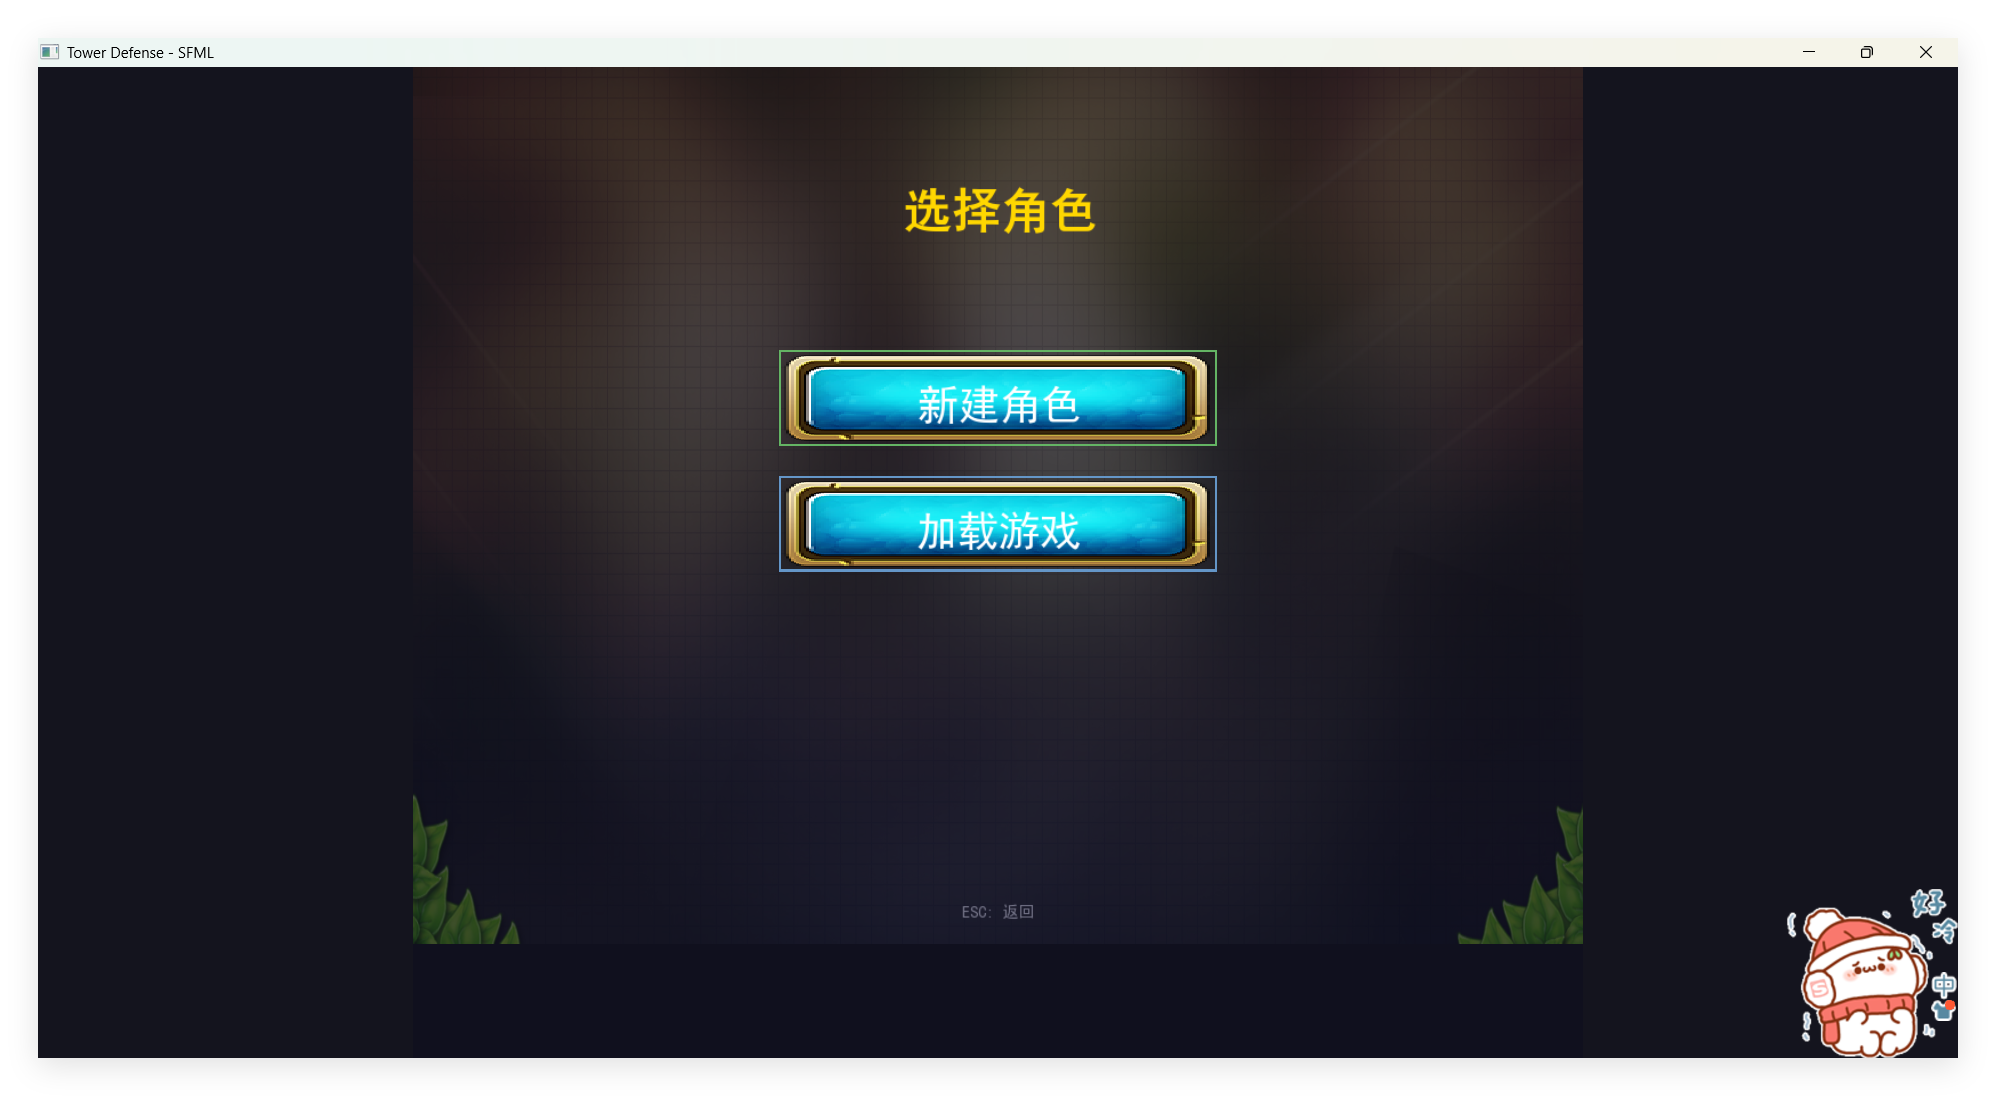
\includegraphics[width=\textwidth]{character_select.png}
        \caption{角色选择界面}
    \end{subfigure}
    \hfill  % 在两个子图之间插入水平空白，让它们分开
    \begin{subfigure}[b]{0.45\textwidth}
        \centering
        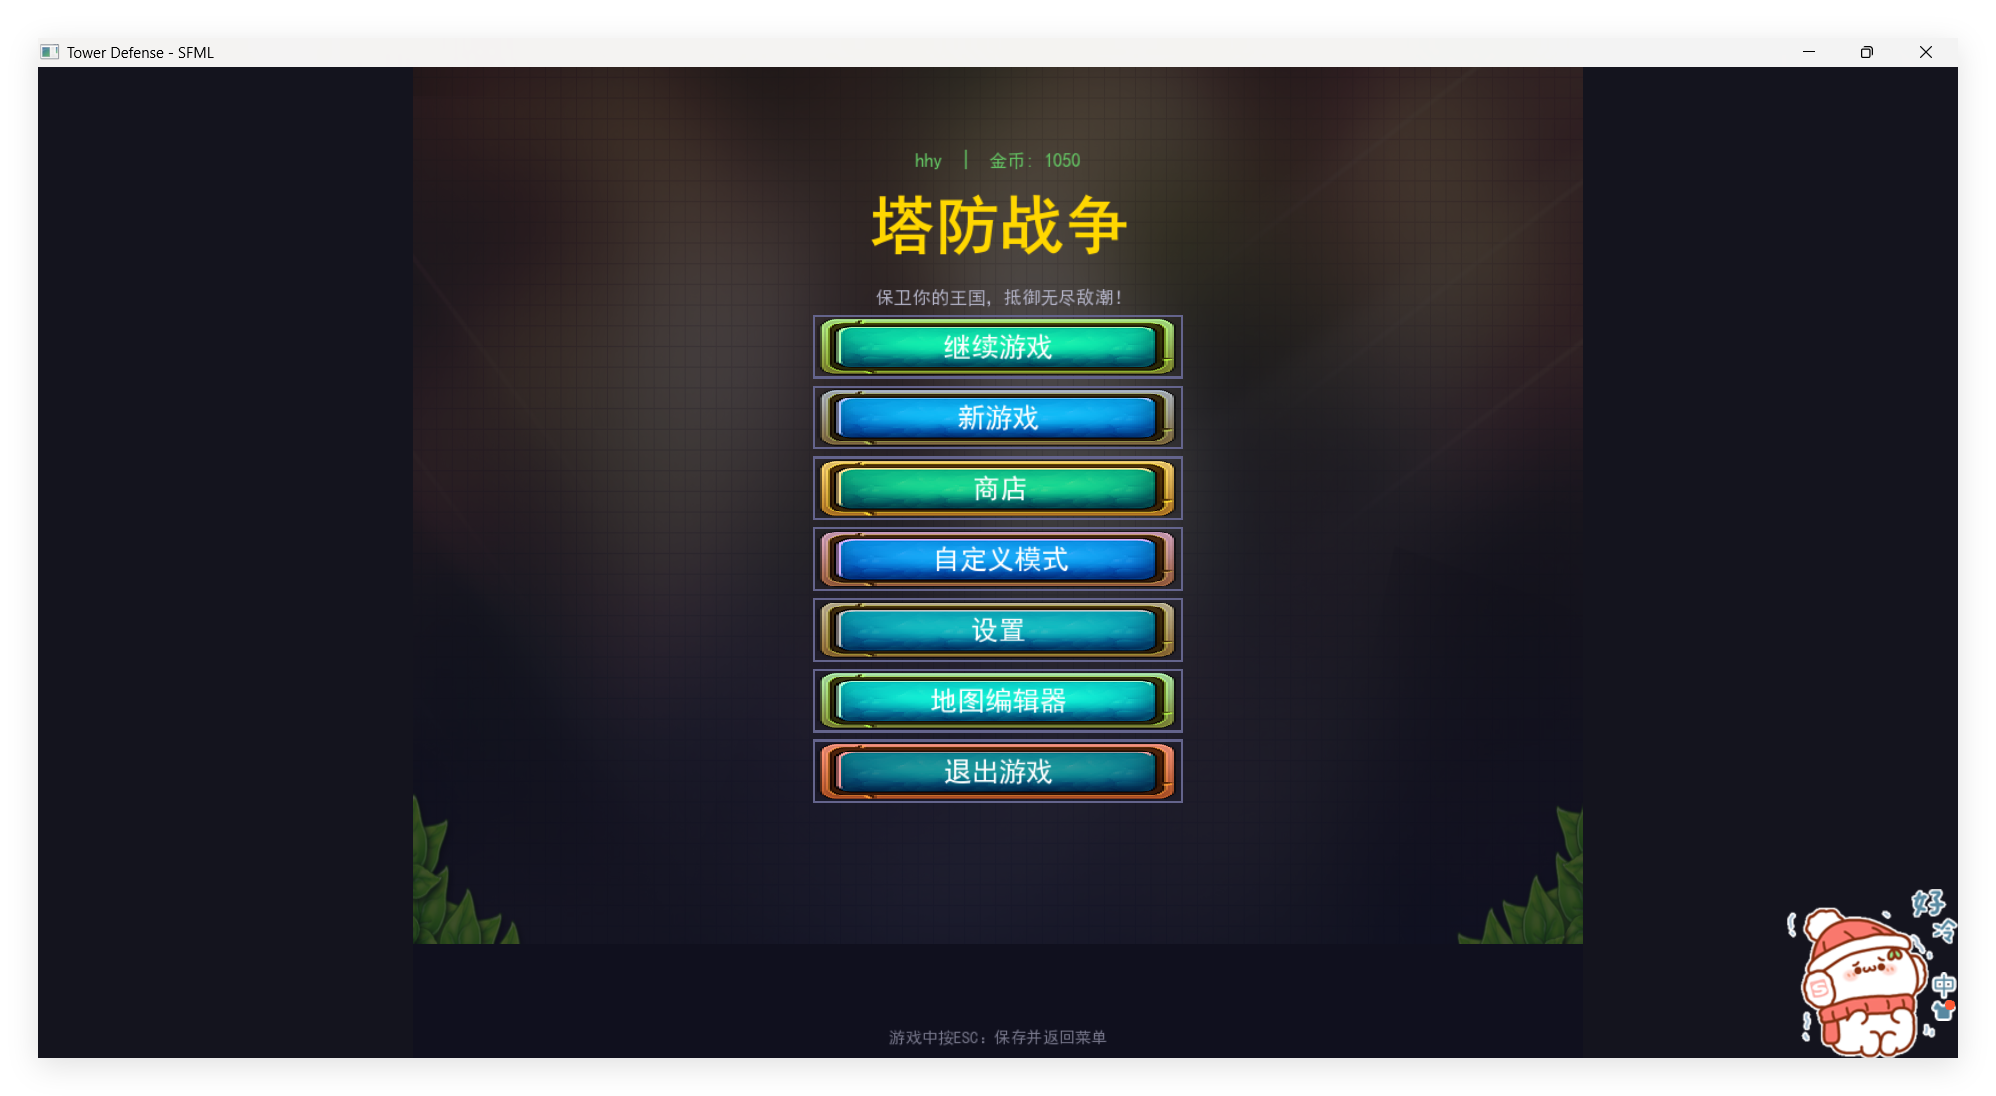
\includegraphics[width=\textwidth]{menu.png}
        \caption{主菜单界面}
    \end{subfigure}
    \caption{游戏界面示例}  % 可选：整个 figure 的大标题
\end{figure}


\section{核心类架构}

\begin{lstlisting}[caption={核心类关系概览}]
Game (主控)
  |-- Map (地图/路径/宝藏)
  |-- UI (界面/消息)
  |-- WaveManager (波次生成)
  |-- Tower 容器 (vector<shared_ptr<Tower>>)
  |-- Enemy 容器 (vector<shared_ptr<Enemy>>)
  |-- Projectile 容器 (vector<shared_ptr<Projectile>>)
  |-- PlayerData (角色/商店数据)
  |-- CampaignScreen (战役选关UI)
  |-- CustomScreen (自定义设置UI)
  |-- LangManager (静态多语言管理)
\end{lstlisting}

\subsection{Game（主控类）}

\texttt{Game} 类是所有逻辑的中心。它有窗口、视图、所有游戏对象的容器以及状态管理。

核心方法分组：
\begin{itemize}
    \item \textbf{生命周期}: \texttt{run()}, \texttt{processEvents()}, \texttt{update()}, \texttt{render()}
    \item \textbf{游戏逻辑}: \texttt{updateTowers()}, \texttt{updateEnemies()}, \texttt{updateProjectiles()}, \texttt{towerFindTargets()}, \texttt{checkProjectileCollisions()}
    \item \textbf{塔操作}: \texttt{handleTowerPlacement()}, \texttt{handleTowerSelection()}, \texttt{handleSellTower()}, \texttt{handleTowerUpgrade()}
    \item \textbf{弹出菜单}: \texttt{showBuildPopup()}, \texttt{showTowerPopup()}, \texttt{drawPopup()}
    \item \textbf{作弊码}: \texttt{processCheatInput()}, \texttt{activateCheat()}
    \item \textbf{存档}: \texttt{newGame()}, \texttt{saveGame()}, \texttt{loadGame()}
\end{itemize}

\begin{figure}[H]
    \centering
    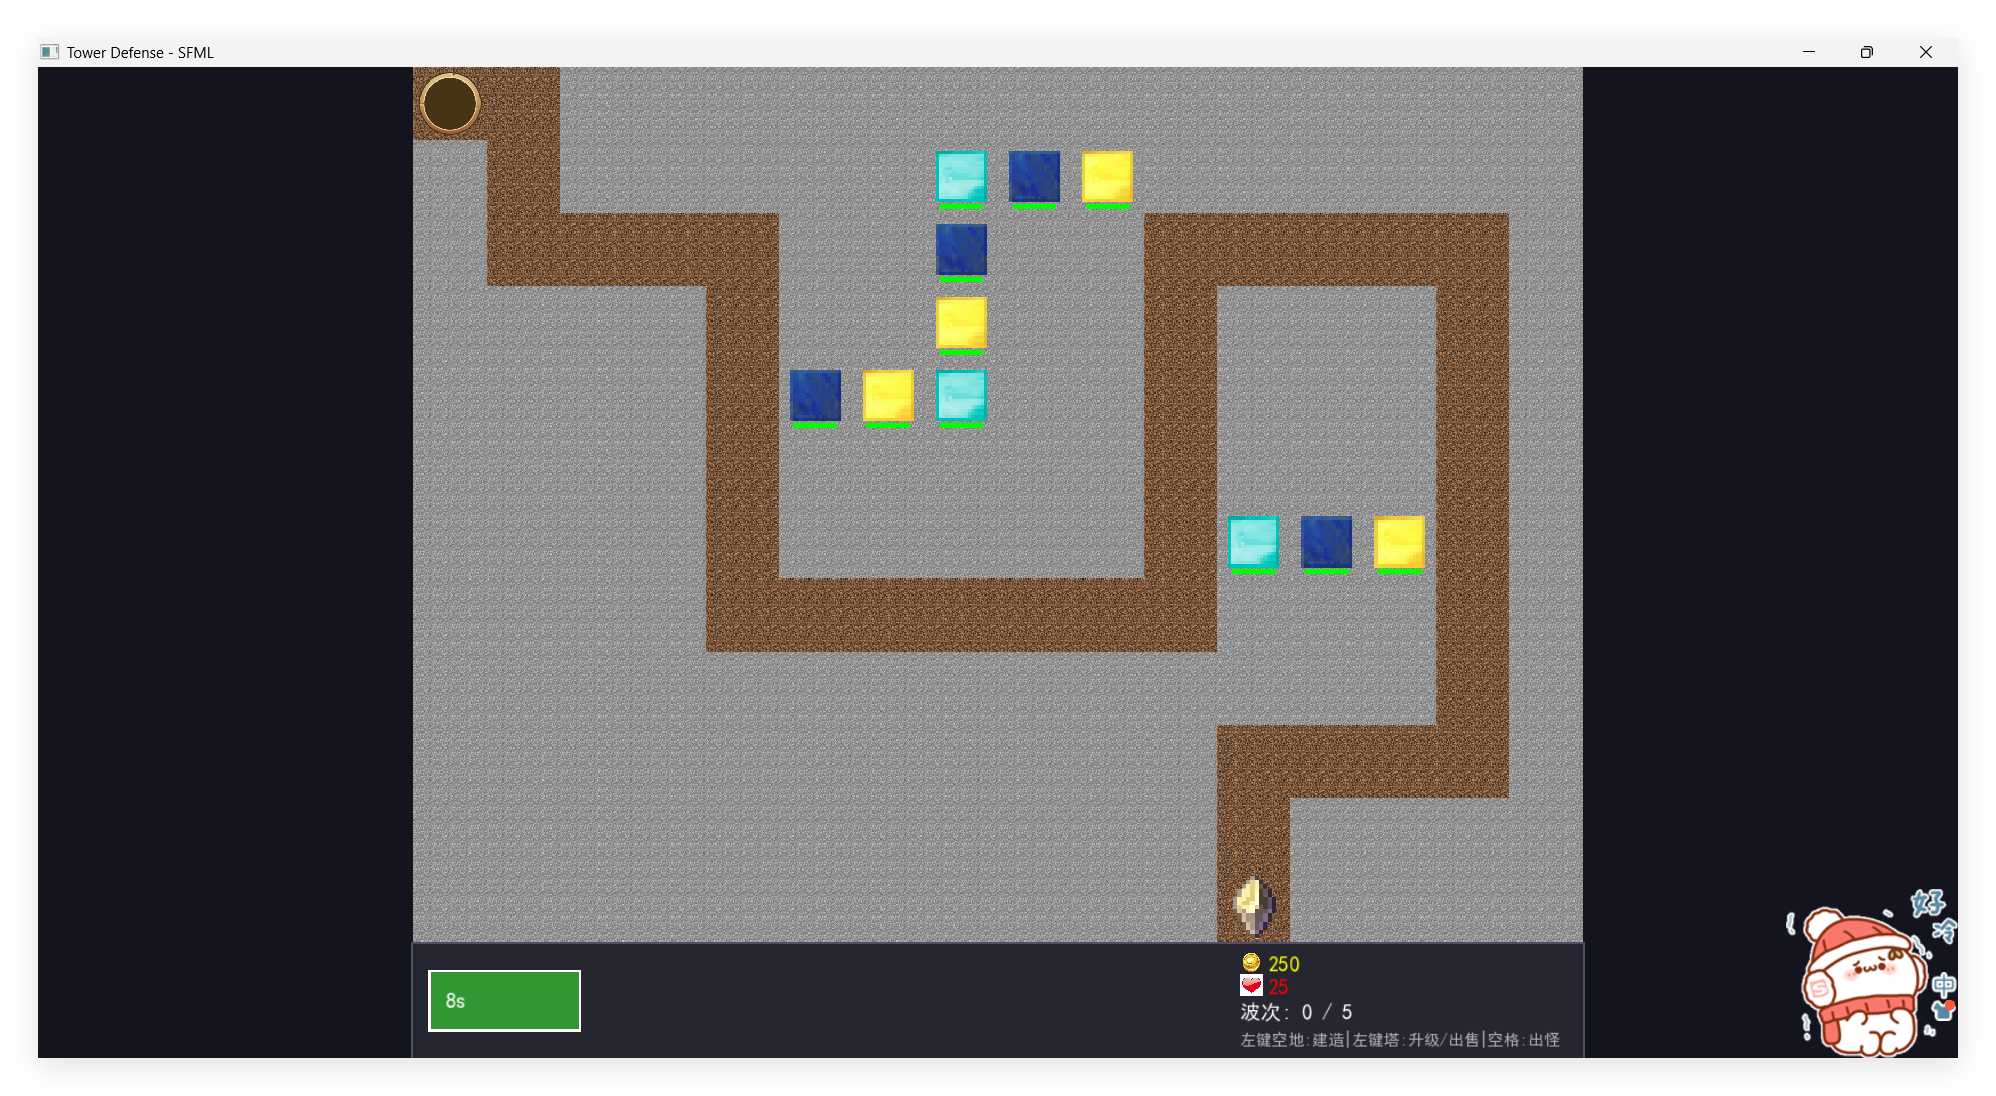
\includegraphics[width=0.7\textwidth]{gameplay.png}
    \caption{游戏进行中画面}
\end{figure}


\section{塔系统}

\subsection{塔类型}

三种基础塔类型，每种都有不同的定位：

\begin{table}[H]
    \centering
    \caption{三种塔类型的基础属性}
    \begin{tabularx}{\textwidth}{lXXXX}
        \toprule
        \textbf{属性} & \textbf{箭塔 (Arrow)} & \textbf{炮塔 (Cannon)} & \textbf{冰塔 (Ice)} \\
        \midrule
        基础费用   & 50   & 100  & 75   \\
        基础射程   & 150  & 120  & 130  \\
        基础伤害   & 15   & 50   & 8    \\
        基础攻速   & 2.0/s & 0.8/s & 1.5/s \\
        颜色       & 绿色  & 红色  & 蓝色  \\
        定位       & 均衡输出 & 高伤害低攻速 & 减速控制 \\
        \bottomrule
    \end{tabularx}
\end{table}

\subsection{升级系统}

每个塔有 3 个等级（Level 1~3），升级效果如下：

\begin{itemize}
    \item 伤害 = 基础伤害 × (1 + (等级-1) × 0.6)
    \item 射程、攻速每级有小幅线性增长
    \item 升级费用 = 下一级造价的 50\%
    \item 售价 = 各级造价之和 × 3/5（约 60\% 返还）
\end{itemize}

\subsection{攻击机制}

\begin{enumerate}
    \item 每帧调用 \texttt{towerFindTargets()} 遍历所有塔
    \item 每个塔寻找射程内最近的存活敌人
    \item 找到目标后：炮口旋转指向目标（冰塔不旋转），创建 \texttt{Projectile} 弹丸，重置射击计时器
    \item 弹丸飞行到目标位置后，调用 \texttt{takeDamage()} 造成伤害
    \item 冰塔击中敌人额外施加减速效果（减速 60\%，持续 2 秒）
\end{enumerate}

\begin{lstlisting}[caption={Game::towerFindTargets()——塔目标选择核心逻辑}]
void Game::towerFindTargets()
{
    float dmgMul = 1.0f, rangeMul = 1.0f, frMul = 1.0f;
    if (m_hasCharacter)
    {
        dmgMul = 1.0f + m_playerData.getDamageBoost();
        rangeMul = 1.0f + m_playerData.getRangeBoost();
        frMul = 1.0f + m_playerData.getFireRateBoost();
    }

    for (auto &tower : m_towers)
    {
        if (!tower->canFire()) continue;

        // 找射程内最近的敌人
        std::shared_ptr<Enemy> bestTarget = nullptr;
        float range = tower->getRange() * rangeMul;
        float bestDist = range;
        for (auto &enemy : m_enemies)
        {
            if (enemy->isDead() || enemy->hasReachedEnd()) continue;
            float dx = enemy->getPosition().x - tower->getPosition().x;
            float dy = enemy->getPosition().y - tower->getPosition().y;
            float dist = std::sqrt(dx * dx + dy * dy);
            if (dist <= range && (!bestTarget || dist < bestDist))
                bestTarget = enemy;
        }
        // 转向 → 发射弹丸 → 重置冷却
        if (bestTarget) {
            tower->setTargetAngle(/* 计算角度 */);
            m_projectiles.push_back(std::make_shared<Projectile>(
                tower->getPosition(), bestTarget,
                tower->getDamage() * dmgMul, 300.0f, tower->getType()));
            tower->resetFireTimer();
        }
    }
}
\end{lstlisting}

\subsection{宝藏攻击机制}

\begin{itemize}
    \item 玩家可以左键点击地图上的宝藏方块
    \item 被点击的宝藏被标记为优先目标
    \item 所有在射程内的塔会将火力转向该宝藏（冰塔除外）
    \item 宝藏被摧毁后返还金币
    \item 宝藏被打后显示血条
\end{itemize}
\begin{figure}[H]
    \centering
    \begin{subfigure}[b]{0.45\textwidth}
        \centering
        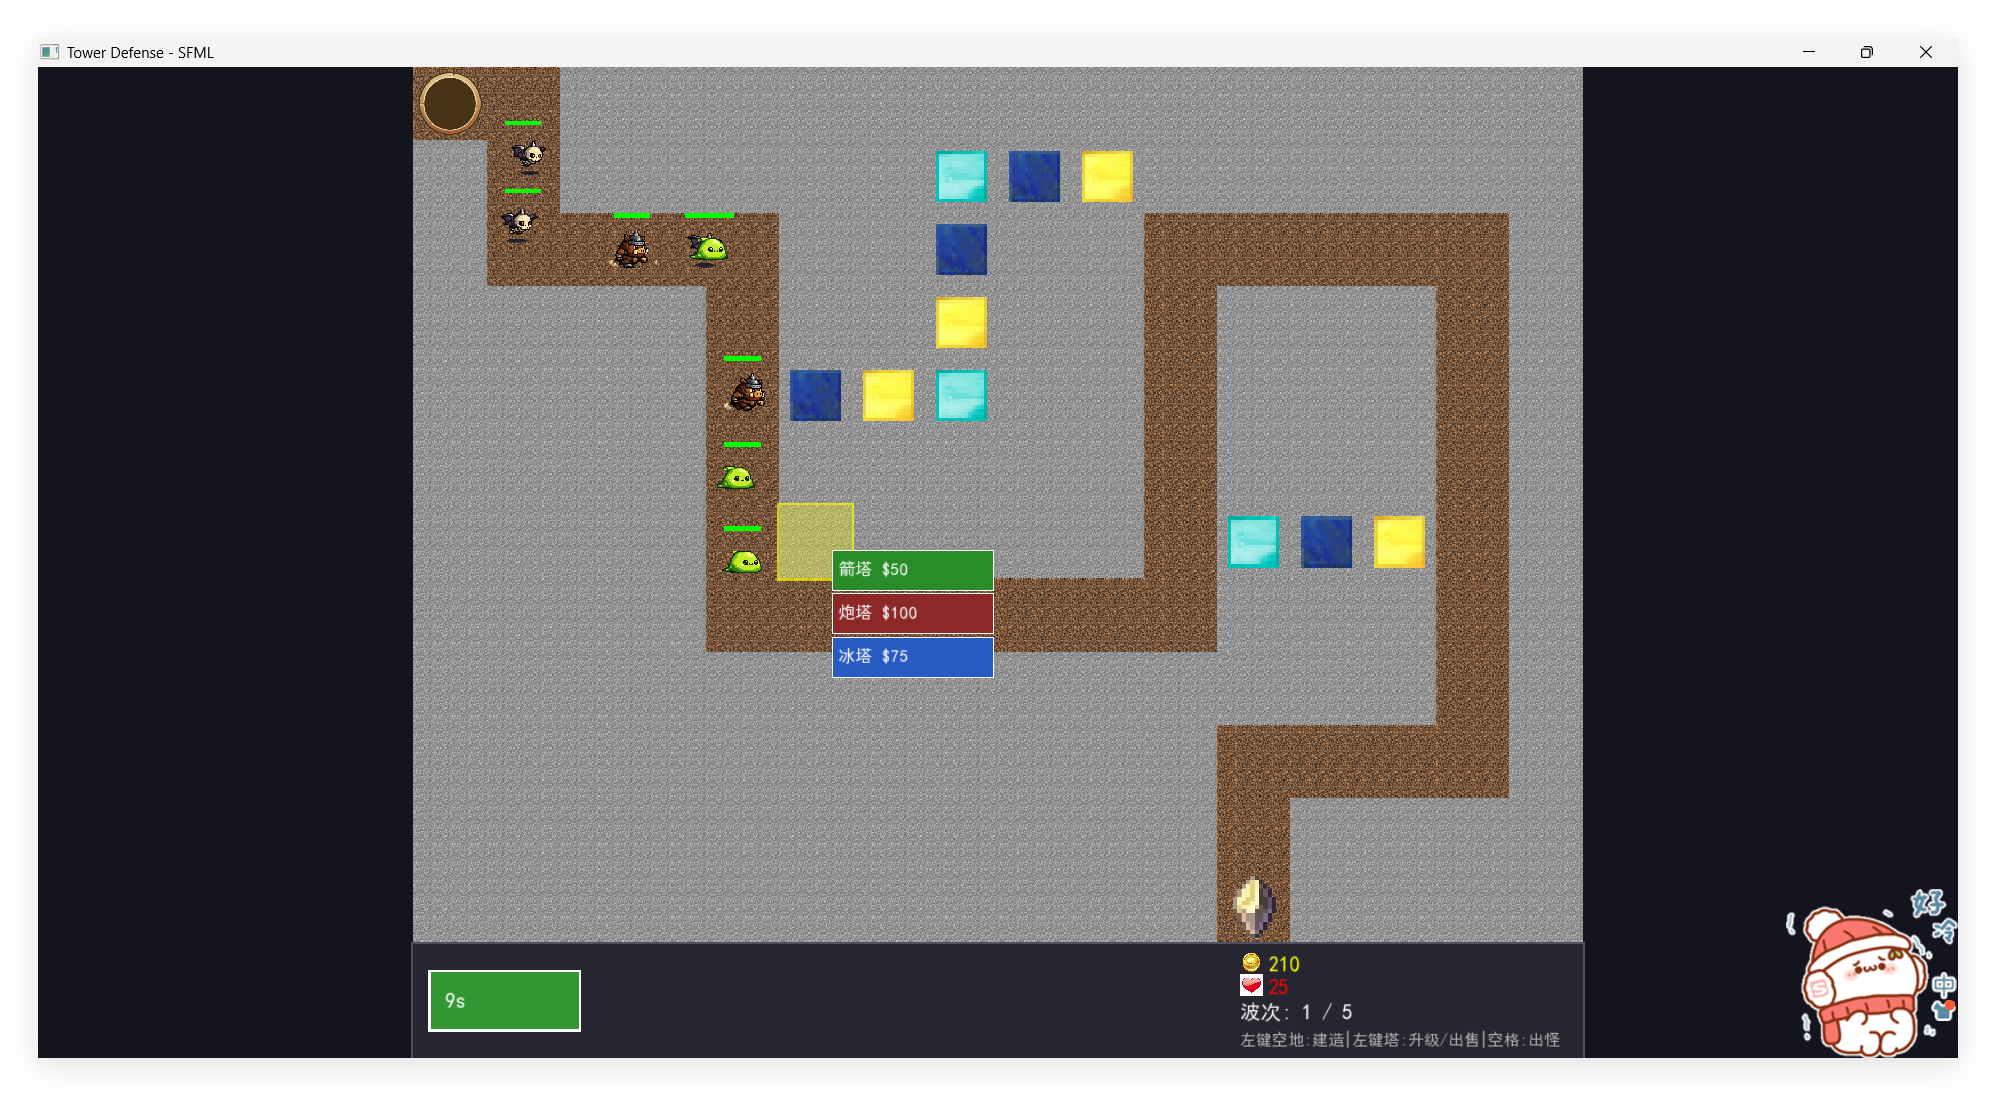
\includegraphics[width=\textwidth]{build_popup.png}
        \caption{建造弹窗——点击空地后选择塔类型}
    \end{subfigure}
    \hfill  % 在两个子图之间插入水平空白，让它们分开
    \begin{subfigure}[b]{0.45\textwidth}
        \centering
        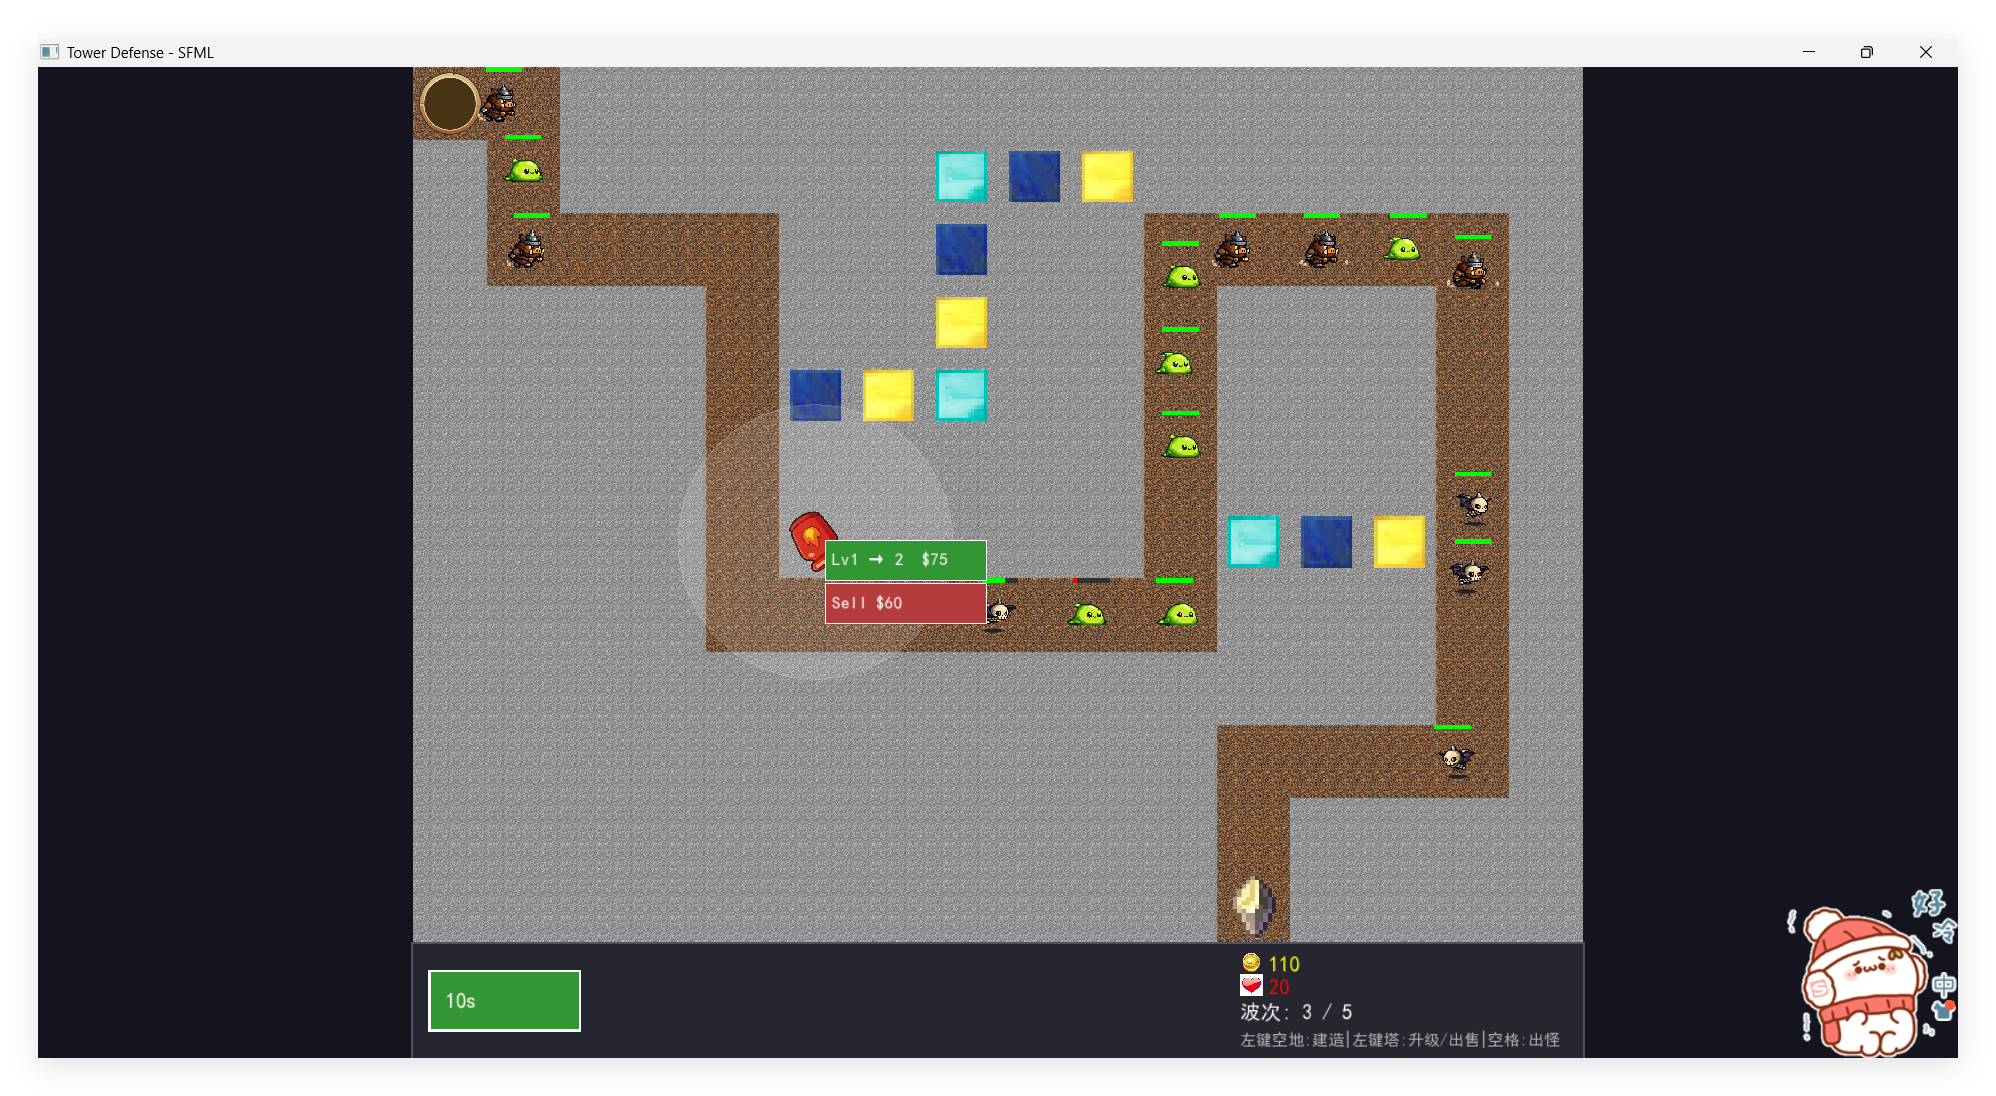
\includegraphics[width=\textwidth]{tower_popup.png}
        \caption{塔管理弹窗——升级与出售}
    \end{subfigure}
    \caption{游戏弹窗}  % 可选：整个 figure 的大标题
\end{figure}

\section{敌人系统}

\subsection{敌人变体}

敌人系统使用纹理变体（Variant）机制实现不同类型的敌人：

\begin{table}[H]
    \centering
    \caption{敌人变体配置}
    \begin{tabularx}{\textwidth}{lXXXXX}
        \toprule
        \textbf{名称} & \textbf{HP倍率} & \textbf{速度倍率} & \textbf{金币倍率} & \textbf{权重} & \textbf{类型} \\
        \midrule
        绿色史莱姆  & 1.0  & 1.0  & 1 & 40 & 普通 \\
        黄色中型    & 1.6  & 1.0  & 1 & 35 & 普通 \\
        红色重型    & 2.5  & 0.8  & 2 & 25 & 普通 \\
        BOSS 1      & 5.0  & 0.5  & 3 & 0  & Boss \\
        BOSS 2      & 6.0  & 0.4  & 4 & 0  & Boss \\
        \bottomrule
    \end{tabularx}
\end{table}

\begin{lstlisting}[caption={Enemy::loadTextures()——变体配置数组}]
void Enemy::loadTextures()
{
    struct {
        const char* path;
        float hpMul; float spdMul;
        int rewardMul; int weight;
    } cfg[] = {
        {"textures/enemy1.png", 1.0f, 1.0f, 1, 40},  // 绿色史莱姆
        {"textures/enemy2.png", 1.6f, 1.0f, 1, 35},  // 黄色中型
        {"textures/enemy3.png", 2.5f, 0.8f, 2, 25},  // 红色重型
        {"textures/boss1.png",  5.0f, 0.5f, 3,  0},  // BOSS1
        {"textures/boss2.png",  6.0f, 0.4f, 4,  0},  // BOSS2
    };
    // 加权随机：权重>0的参与普通出怪
    // BOSS 权重为0，只在最后一波用 getRandomBoss() 选取
}
\end{lstlisting}

\begin{itemize}
    \item 普通怪通过加权随机算法选取（权重越大出现概率越高）
    \item Boss 权重为 0，不会在普通波次中出现
    \item Boss 在最后一波随机选取一只生成
\end{itemize}

\subsection{敌人行为}

\begin{enumerate}
    \item 从出生点（TileType::Start）生成
    \item 沿着预计算的路点（Waypoint）序列移动
    \item 到达终点后扣除玩家一条生命并从游戏中移除
    \item HP 归零后变为死亡状态，加金币并移除
    \item 敌人有 4 帧动画（纹理横向切分），根据移动方向翻转精灵
\end{enumerate}

\subsection{减速机制}

冰塔击中敌人后触发：
\begin{itemize}
    \item \texttt{applySlow(factor, duration)} 设置减速系数和持续时间
    \item 减速系数 0.4 = 速度降至 40\%，持续 2 秒
    \item 计时结束后自动恢复
\end{itemize}


\section{波次系统}

\subsection{WaveManager}

\texttt{WaveManager} 负责波次的生成和管理：

\begin{itemize}
    \item 管理波次队列（\texttt{m\_waves}），每个波次包含：敌人数、生成间隔、速度、HP、金币和颜色
    \item 跟踪当前波次索引、已生成数、剩余数
    \item 提供 \texttt{canStartWave()}、\texttt{startNextWave()}、\texttt{isWaveComplete()} 等接口
    \item 支持自定义模式的波次生成：\texttt{setCustomWaves(waveCount, enemiesPerWave, speedMul, hpMul)}
    \item 支持作弊：\texttt{skipToLastWave()} 跳到最后一波，\texttt{forceAllComplete()} 强制通关
\end{itemize}

\subsection{波次流程}

\begin{enumerate}
    \item 初始倒计时 10 秒后自动开始第一波
    \item 玩家也可以通过点击"Start Wave"按钮或按空格键手动开始
    \item 手动开始后续波次时，奖励 50 + (波次-1)×10 金币
    \item 波次中敌人按设定的间隔逐个生成
    \item 当前波次所有敌人被消灭后，可以开始下一波
    \item 所有波次完成且场上无敌人时，游戏胜利
\end{enumerate}

\begin{lstlisting}[caption={WaveManager::setCustomWaves()——动态生成波次}]
void WaveManager::setCustomWaves(int waveCount, int enemiesPerWave,
                                  float speedMul, float hpMul)
{
    for (int i = 0; i < waveCount; ++i)
    {
        WaveData wd;
        wd.enemyCount = enemiesPerWave + i * 2;
        wd.spawnInterval = std::max(0.3f, 1.0f - i * 0.05f);
        wd.speed = (80.0f + i * 5.0f) * speedMul;
        wd.hp = (50.0f + i * 20.0f) * hpMul;
        wd.reward = 10 + i * 3;
        wd.color = colors[i % 8];
        m_waves.push_back(wd);
    }
}
\end{lstlisting}


\section{地图系统}

\subsection{瓦片类型}

\begin{table}[H]
    \centering
    \caption{瓦片类型定义}
    \begin{tabularx}{\textwidth}{clX}
        \toprule
        \textbf{值} & \textbf{类型} & \textbf{描述} \\
        \midrule
        0 & Grass  & 草地，可放置塔 \\
        1 & Path   & 敌人路径 \\
        2 & Start  & 出生点 \\
        3 & End    & 终点 \\
        4 & Blocked & 不可放置（含宝藏） \\
        \bottomrule
    \end{tabularx}
\end{table}

\subsection{路径查找}

\begin{itemize}
    \item 使用 C 接口的路径查找器（\texttt{PathFinder.h / PathFinder.c}）
    \item \texttt{pf\_tracePath()} 从 Start（2）出发沿 Path（1）追踪到 End（3）
    \item 返回路点（Waypoint）序列供敌人跟随
\end{itemize}

\subsection{群系系统}

游戏包含四种群系（Biome），影响地图纹理和关卡：

\begin{itemize}
    \item \textbf{Grassland（翠绿平原）}: ground1.png, kong1.png
    \item \textbf{Desert（沙漠风暴）}: ground2.png, kong2.png
    \item \textbf{Hell（地狱深渊）}: ground3.png, kong3.png
    \item \textbf{Community（社区关卡）}: ground1.png, kong1.png（复用草地纹理）
\end{itemize}

每个群系有自己的地面纹理和装饰纹理，通过 \texttt{loadBiomeTextures()} 和 \texttt{loadKongTexture()} 加载。

\subsection{宝藏系统}

\begin{itemize}
    \item 所有 Blocked 类型的瓦片自动成为宝藏候选
    \item 三种宝藏纹理：Treasure1（50 金币/3 HP）、Treasure2（100 金币/5 HP）、Treasure3（150 金币/8 HP）
    \item 宝藏分配使用确定性哈希：\texttt{(c * 7 + r * 13) \% count}
    \item 被摧毁后所在格子变为 Grass，可以放置塔
    \item 受击后显示血条 3 秒
\end{itemize}

\begin{figure}[H]
    \centering
    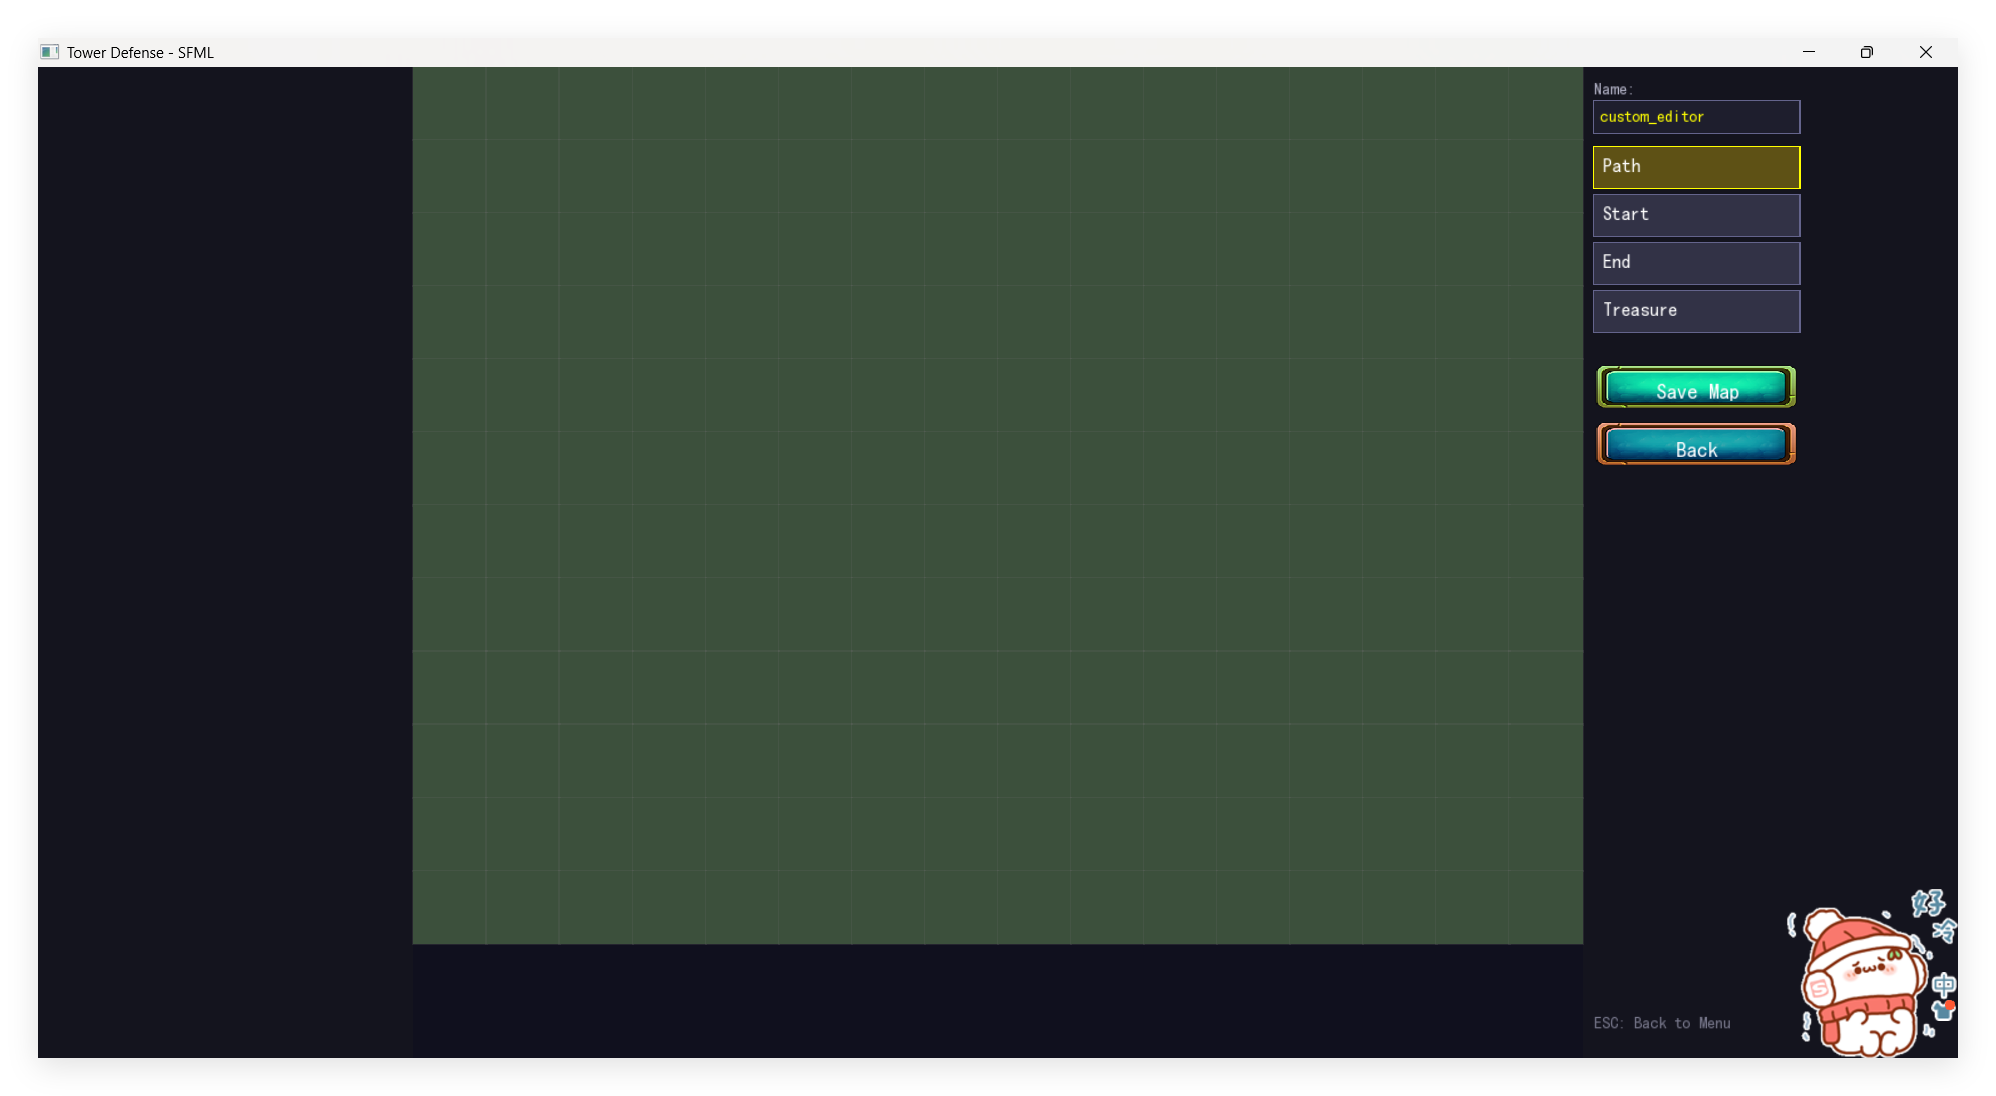
\includegraphics[width=0.7\textwidth]{map_editor.png}
    \caption{内置地图编辑器}
\end{figure}


\section{经济系统}

\subsection{金币来源}

\begin{itemize}
    \item 关卡初始金币（战役配置或自定义设置）
    \item 消灭敌人获得奖励（基础奖励 × 敌人变体倍率）
    \item 手动开始波次奖励（50 + 波次 × 10）
    \item 摧毁宝藏获得金币（50/100/150）
    \item 商店购买"起始金币加成"
    \item 作弊码 "money" 开启无限金币
\end{itemize}

\subsection{金币消耗}

\begin{itemize}
    \item 建造塔（基础造价可享受商店折扣）
    \item 升级塔
    \item 商店购买升级（永久性跨关卡）
\end{itemize}

\subsection{商店系统}

6 种商店升级项目，每个最多 5 级：

\begin{table}[H]
    \centering
    \caption{商店升级项目}
    \begin{tabularx}{\textwidth}{lXX}
        \toprule
        \textbf{项目} & \textbf{每级效果} & \textbf{价格（基础+递增）} \\
        \midrule
        StartGoldBonus & +50 起始金币   & 80 + 40/级 \\
        TowerDiscount  & -10\% 建塔费用 & 100 + 50/级 \\
        DamageBoost    & +15\% 塔伤害   & 120 + 60/级 \\
        RangeBoost     & +8\% 塔射程    & 100 + 50/级 \\
        LivesBonus     & +3 起始生命    & 90 + 45/级 \\
        FireRateBoost  & +10\% 攻速     & 110 + 55/级 \\
        \bottomrule
    \end{tabularx}
\end{table}

\begin{figure}[H]
    \centering
    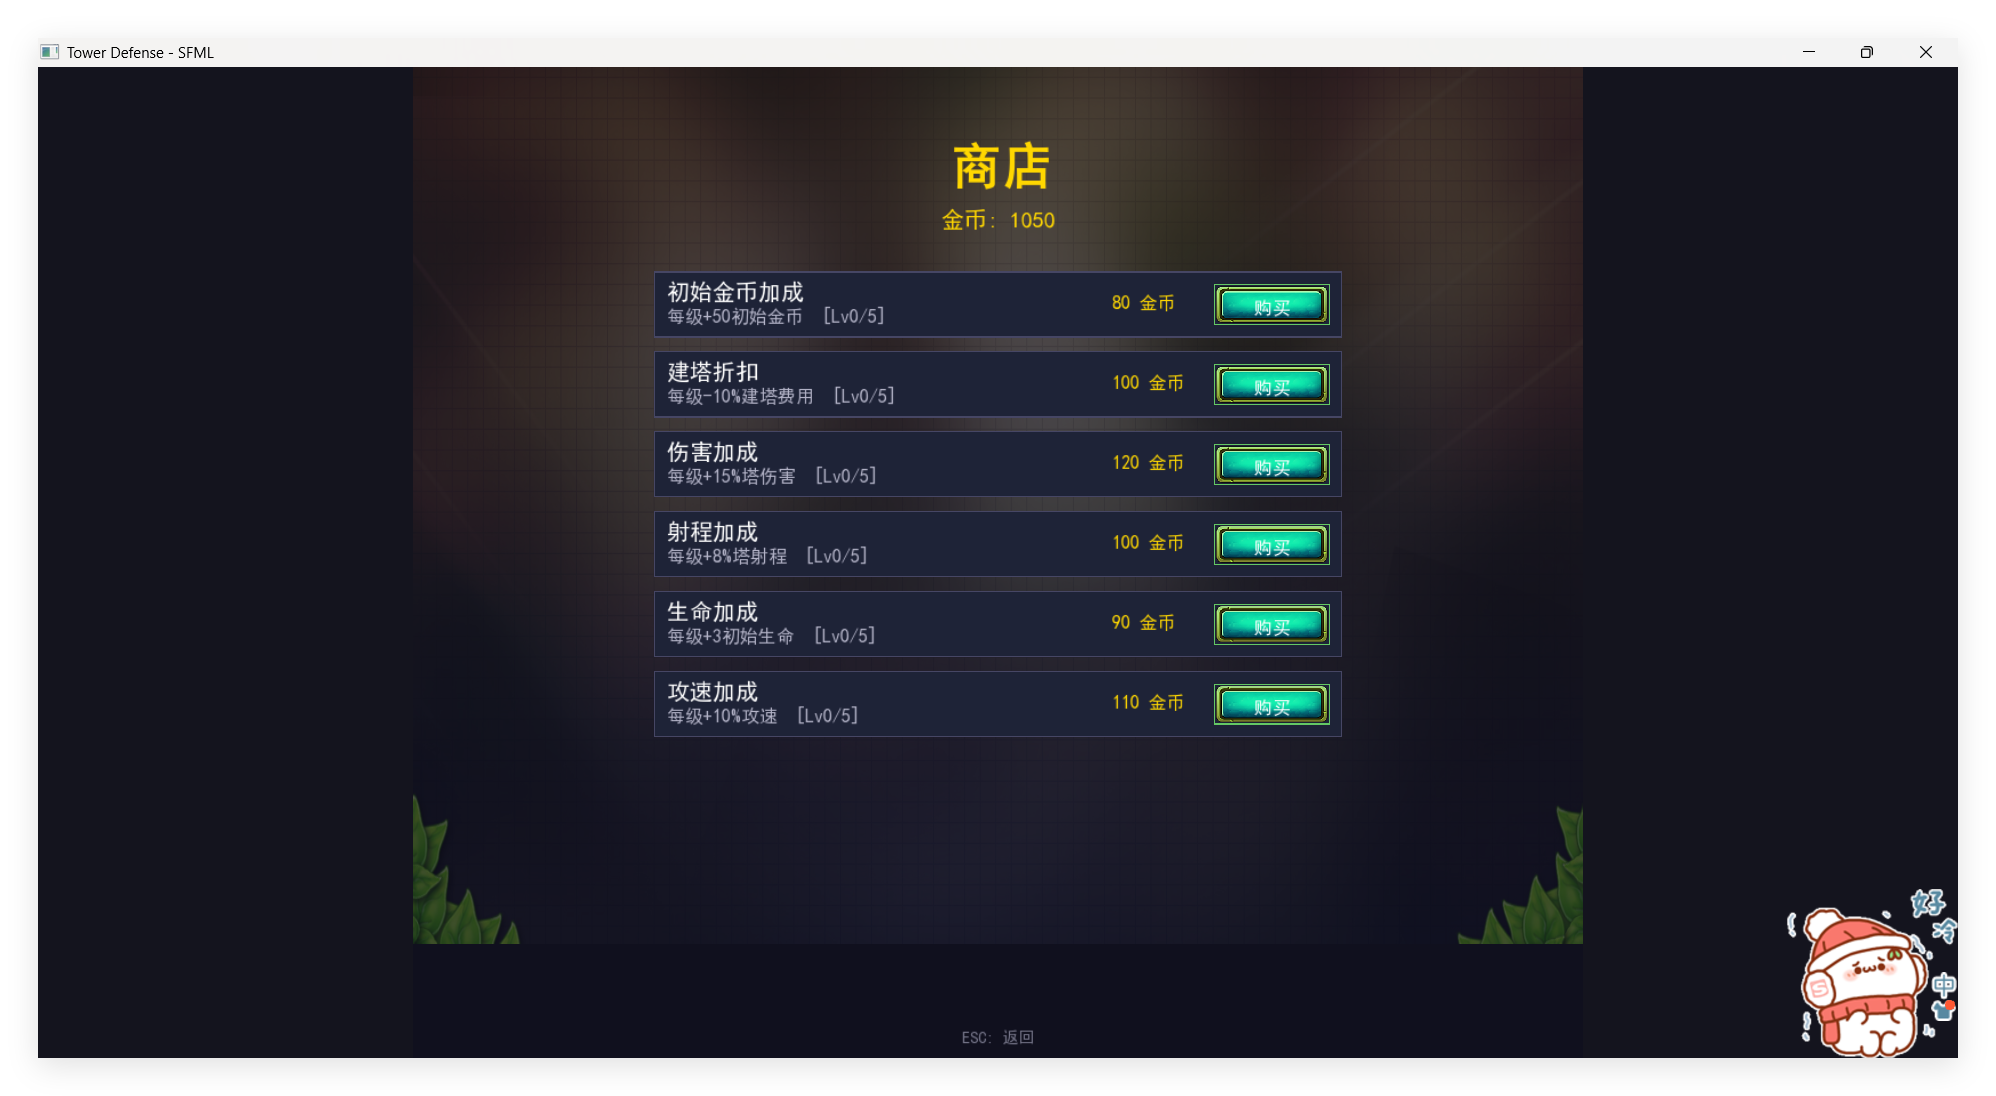
\includegraphics[width=0.7\textwidth]{shop.png}
    \caption{商店升级界面}
\end{figure}


\section{角色与存档系统}

\subsection{角色系统}

玩家创建角色后拥有独立的存档：
\begin{itemize}
    \item 存档路径：根据角色名生成（\texttt{PlayerData::makeSavePath(name)}）
    \item 存档内容：角色名、累计金币、已解锁关卡数、商店等级数组
    \item 支持多角色切换（创建/加载/删除）
    \item 跨关卡累计金币用于商店消费
\end{itemize}

\begin{lstlisting}[caption={PlayerData::save() / load()——二进制存档序列化}]
bool PlayerData::save(const std::string &path) const
{
    std::ofstream f(path, std::ios::binary);
    size_t nameLen = name.size();
    f.write((const char*)&nameLen, sizeof(nameLen));
    f.write(name.data(), nameLen);
    f.write((const char*)&totalGold, sizeof(totalGold));
    f.write((const char*)&unlockedLevels, sizeof(unlockedLevels));
    for (int i = 0; i < SHOP_ITEM_COUNT; ++i)
        f.write((const char*)&shopLevels[i], sizeof(shopLevels[i]));
    return f.good();
}

bool PlayerData::load(const std::string &path)
{
    std::ifstream f(path, std::ios::binary);
    size_t nameLen;
    f.read((char*)&nameLen, sizeof(nameLen));
    name.resize(nameLen);
    f.read(&name[0], nameLen);
    f.read((char*)&totalGold, sizeof(totalGold));
    f.read((char*)&unlockedLevels, sizeof(unlockedLevels));
    for (int i = 0; i < SHOP_ITEM_COUNT; ++i)
        f.read((char*)&shopLevels[i], sizeof(shopLevels[i]));
    return f.good();
}
\end{lstlisting}

\subsection{通关与解锁}

\begin{itemize}
    \item 关卡胜利时累计金币至角色存档
    \item 若当前关卡是最后解锁的关卡，自动解锁下一关
    \item 社区关卡（Community）不计入主线进度
    \item 商店升级跨关卡保留
\end{itemize}


\section{战役与自定义模式}

\subsection{战役模式}

\begin{table}[H]
    \centering
    \caption{战役关卡配置（难度系数列 = 速度倍率/HP倍率）}
    \begin{tabularx}{\textwidth}{clllll}
        \toprule
        \textbf{关卡} & \textbf{群系} & \textbf{起始金币} & \textbf{起始生命} & \textbf{波次} & \textbf{难度系数} \\
        \midrule
        1-1 & Grassland & 250 & 25 & 5 & 0.9/0.8 \\
        1-2 & Grassland & 220 & 22 & 6 & 1.0/0.9 \\
        1-3 & Grassland & 200 & 20 & 7 & 1.1/1.0 \\
        2-1 & Desert    & 200 & 20 & 7 & 1.1/1.2 \\
        2-2 & Desert    & 180 & 18 & 8 & 1.2/1.4 \\
        2-3 & Desert    & 160 & 16 & 9 & 1.3/1.6 \\
        3-1 & Hell      & 180 & 18 & 8 & 1.3/1.5 \\
        3-2 & Hell      & 160 & 16 & 9 & 1.5/1.8 \\
        3-3 & Hell      & 140 & 14 & 10 & 1.7/2.0 \\
        c1  & Community & 300 & 30 & 8 & 1.0/0.9 \\
        c2  & Community & 250 & 25 & 10 & 1.2/1.1 \\
        \bottomrule
    \end{tabularx}
\end{table}

\begin{figure}[H]
    \centering
    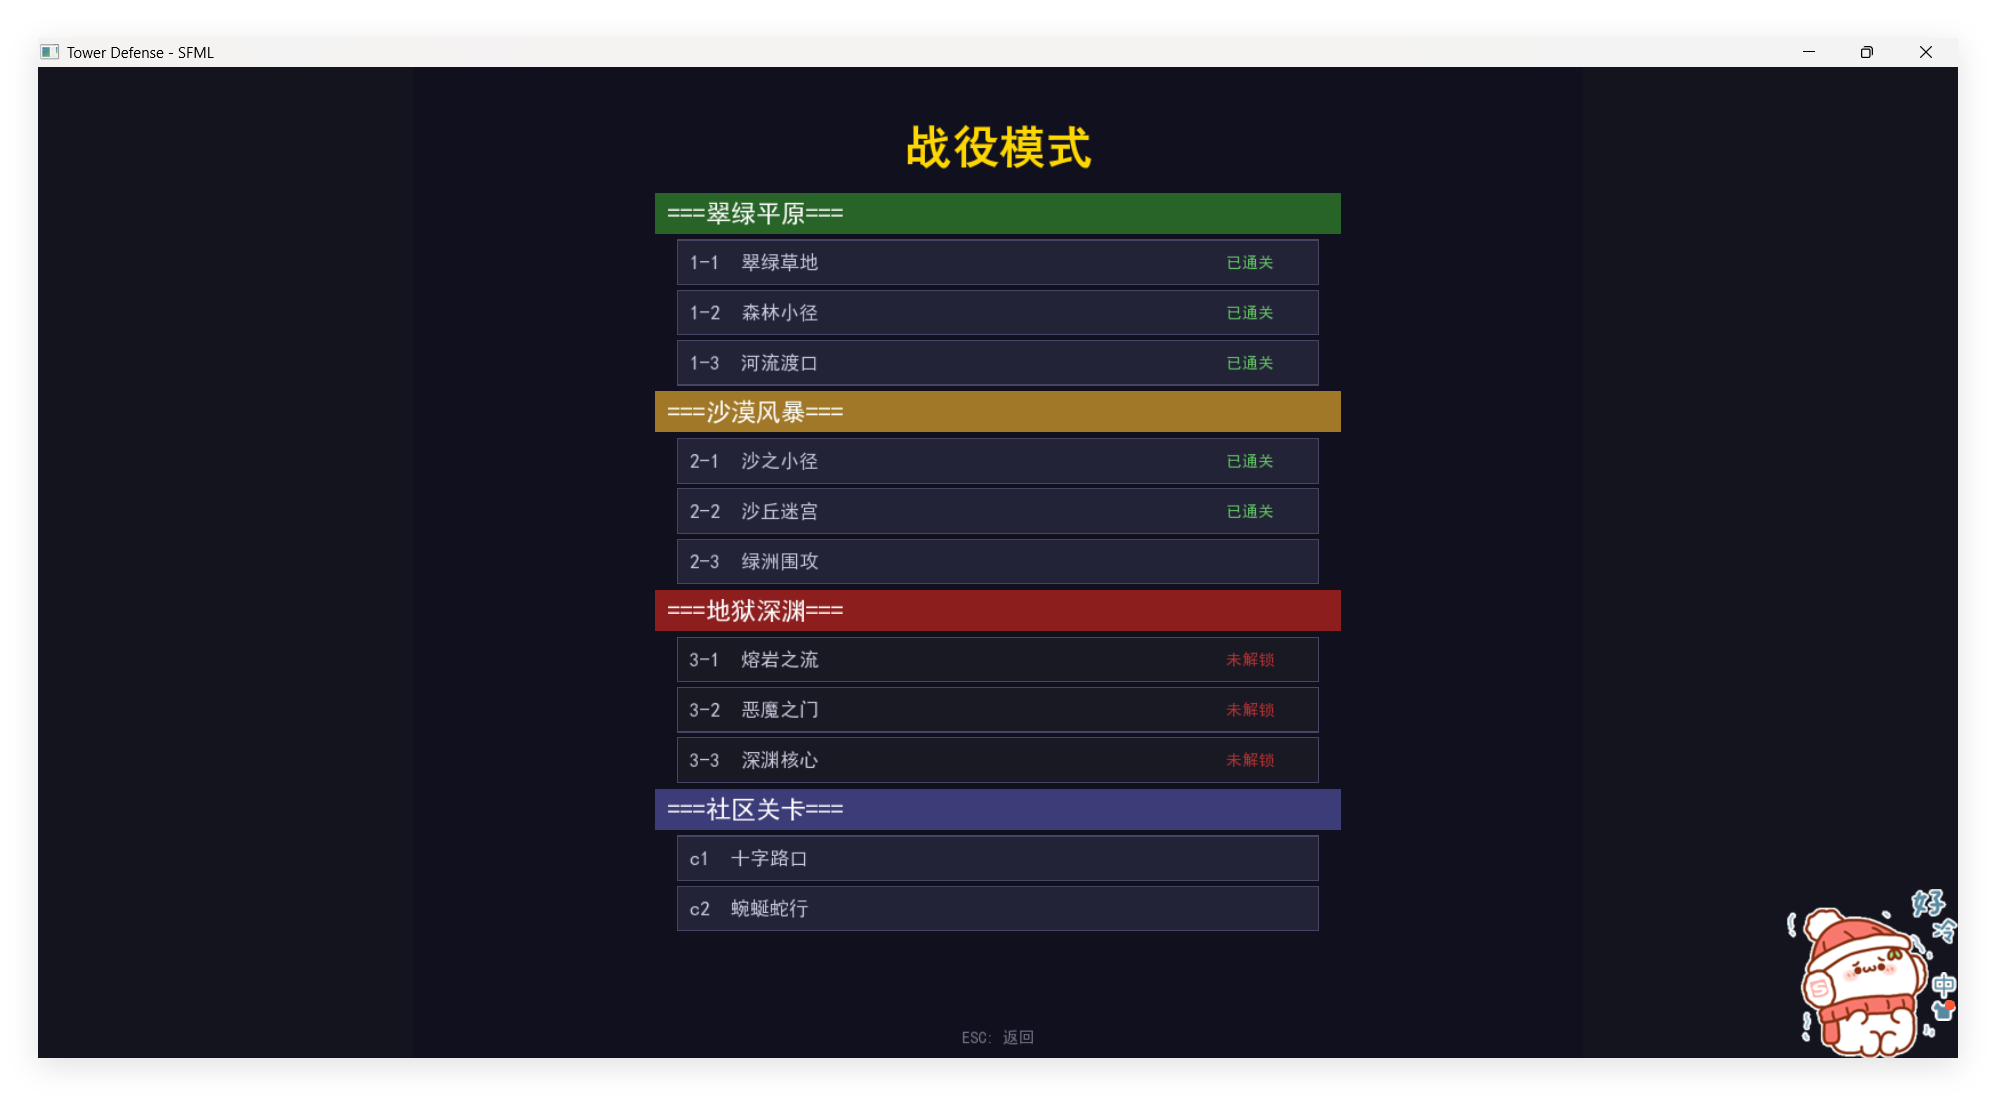
\includegraphics[width=0.7\textwidth]{campaign.png}
    \caption{战役选关界面}
\end{figure}

\subsection{自定义模式}

玩家可以自定义以下参数：
\begin{itemize}
    \item 波次数量（Waves）
    \item 每波敌人数（Enemies/Wave）
    \item 起始金币（Start Gold）
    \item 起始生命（Start Lives）
    \item 速度倍率（Speed Multiplier）
    \item HP 倍率（HP Multiplier）
    \item 地图选择（从可用列表中选取）
\end{itemize}

\begin{figure}[H]
    \centering
    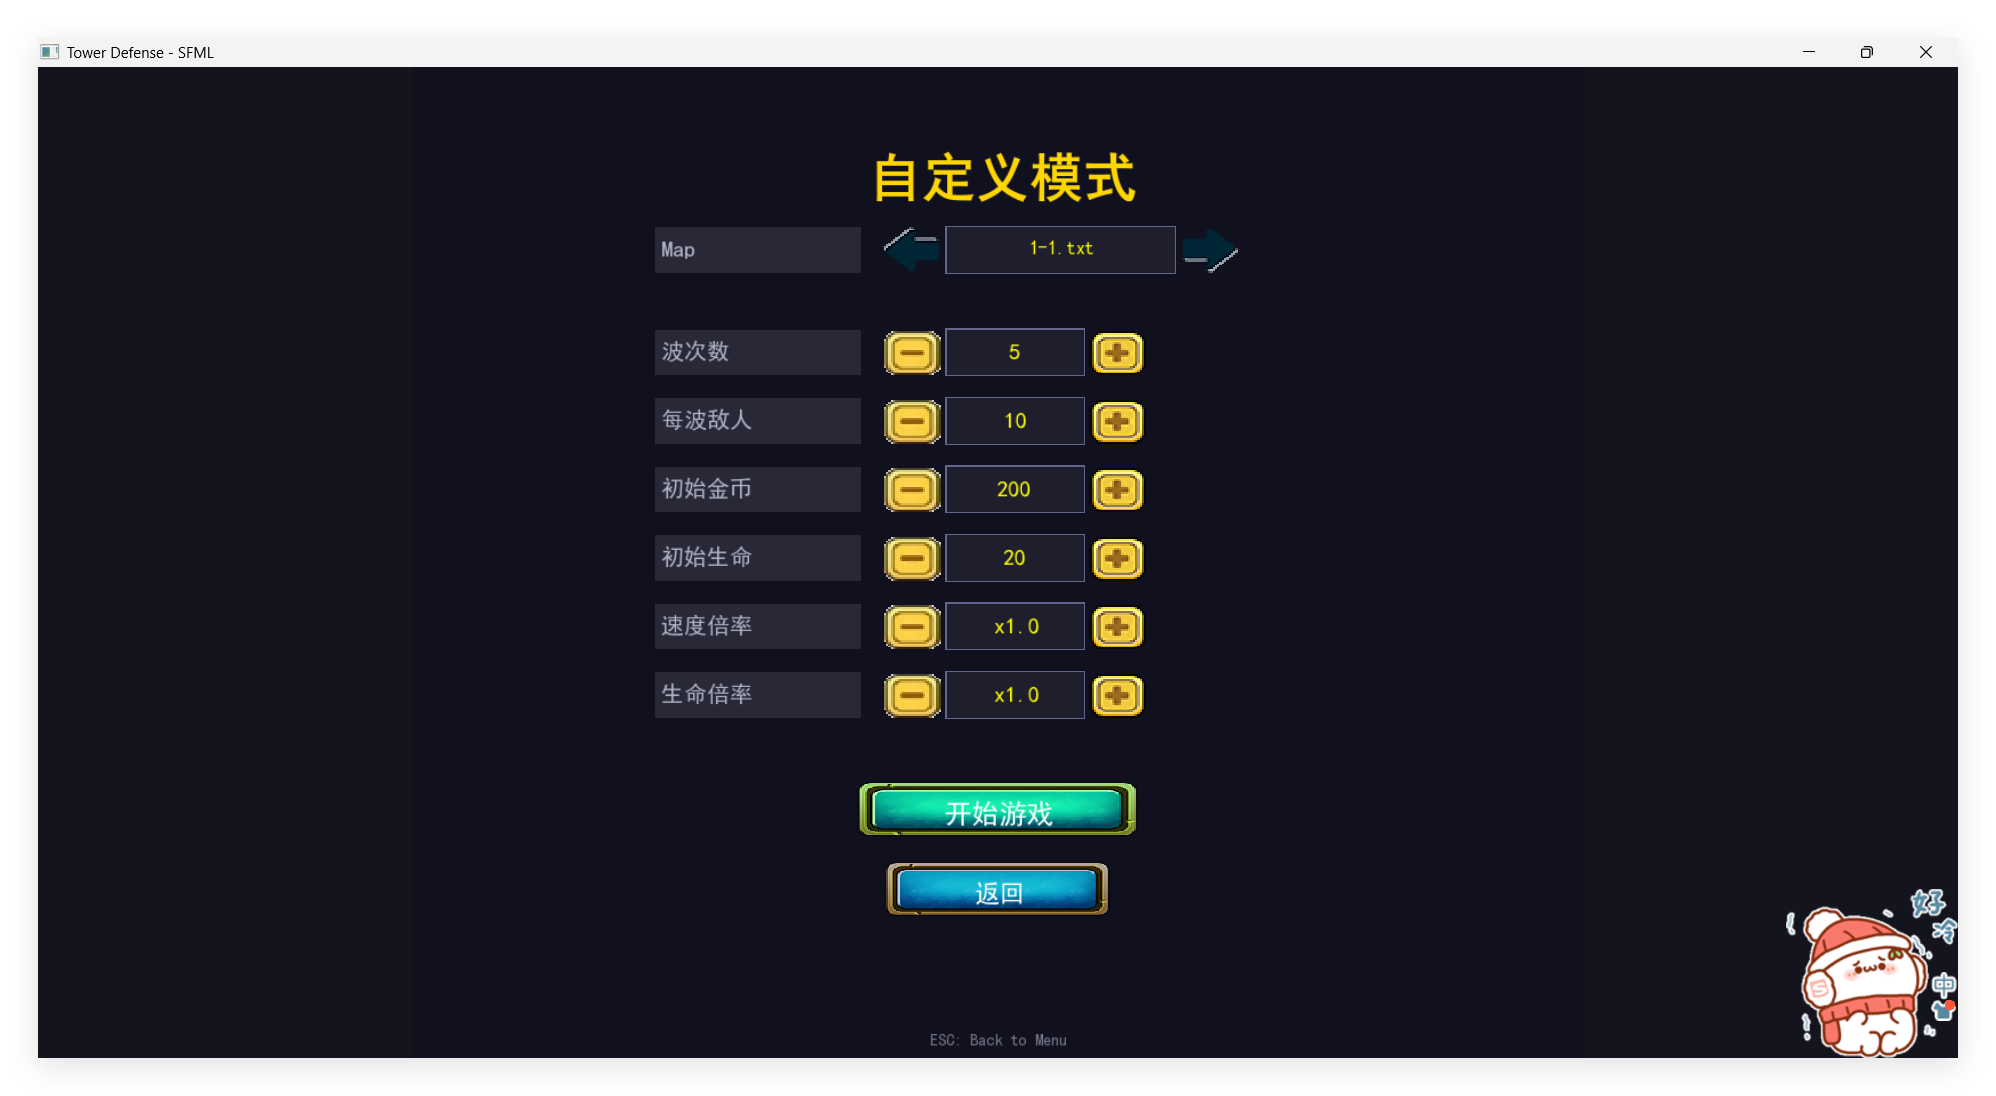
\includegraphics[width=0.7\textwidth]{custom_setup.png}
    \caption{自定义模式参数设置}
\end{figure}


\section{UI 系统}

\subsection{游戏内 HUD}

\begin{itemize}
    \item 信息栏：金币、生命值、当前波次/总波次
    \item 塔选择按钮：箭塔/炮塔/冰塔（显示名称和造价）
    \item "Start Wave" 按钮：手动开始下一波
    \item 游戏提示信息（消息气泡，自动消失）
\end{itemize}

\subsection{弹出菜单}

\textbf{建造弹窗}：
\begin{itemize}
    \item 点击空地（Grass）时显示
    \item 列出三种塔及其造价
    \item 同时高亮目标格子
    \item 检查金币是否充足、位置是否可建造
\end{itemize}

\textbf{塔管理弹窗}：
\begin{itemize}
    \item 点击已有塔时显示
    \item 升级按钮（显示当前等级→下一级 + 费用，满级显示 MAX）
    \item 出售按钮（显示回收价格）
\end{itemize}

\subsection{暂停菜单}

游戏进行中按 Esc 键暂停，显示：
\begin{itemize}
    \item 继续游戏
    \item 保存并返回主菜单
    \item 暂停时游戏逻辑不更新
\end{itemize}

\subsection{语言系统}

游戏支持中英文动态切换，无需重启。

\subsubsection{架构设计}

\texttt{LangManager} 是一个静态类，所有数据通过静态成员管理：

\begin{itemize}
    \item \texttt{s\_currentLang} — 当前语言名称（如 \texttt{"en"}、\texttt{"zh"}）
    \item \texttt{s\_fontPath} — 当前语言对应的字体路径
    \item \texttt{s\_texts[\,]} — 固定大小的 \texttt{std::wstring} 数组，以 \texttt{TextKey} 枚举为索引
    \item \texttt{KEY\_MAP[\,]} — 字符串名称到 \texttt{TextKey} 枚举的映射表
\end{itemize}

\subsubsection{JSON 语言文件}

采用扁平 JSON 格式，每个 key 对应一个字符串值。key 通过 \texttt{KEY\_MAP} 映射表转换为 \texttt{TextKey} 枚举，填入 \texttt{s\_texts[\,]} 数组。中文版（\texttt{lang\_zh.json}）使用相同的 key，value 替换为中文文本，并将 \texttt{Font} 指向中文字体 \texttt{simhei.ttf}。

加载流程：读取 JSON → 内置状态机解析器 → 遍历 KEY\_MAP 填入数组 → 提取字体路径 → 文件名识别语言名。

\subsubsection{语言切换}

设置界面通过左右箭头切换语言，调用 \texttt{LangManager::loadLanguage()} 加载新 JSON，再通过 \texttt{refreshAllTexts()} 重建所有界面文本。SFML 的 \texttt{sf::Text} 使用 \texttt{std::wstring}，JSON 中的 UTF-8 字符串通过 Windows \texttt{MultiByteToWideChar} 转码。

\begin{figure}[H]
    \centering
    \begin{subfigure}[b]{0.45\textwidth}
        \centering
        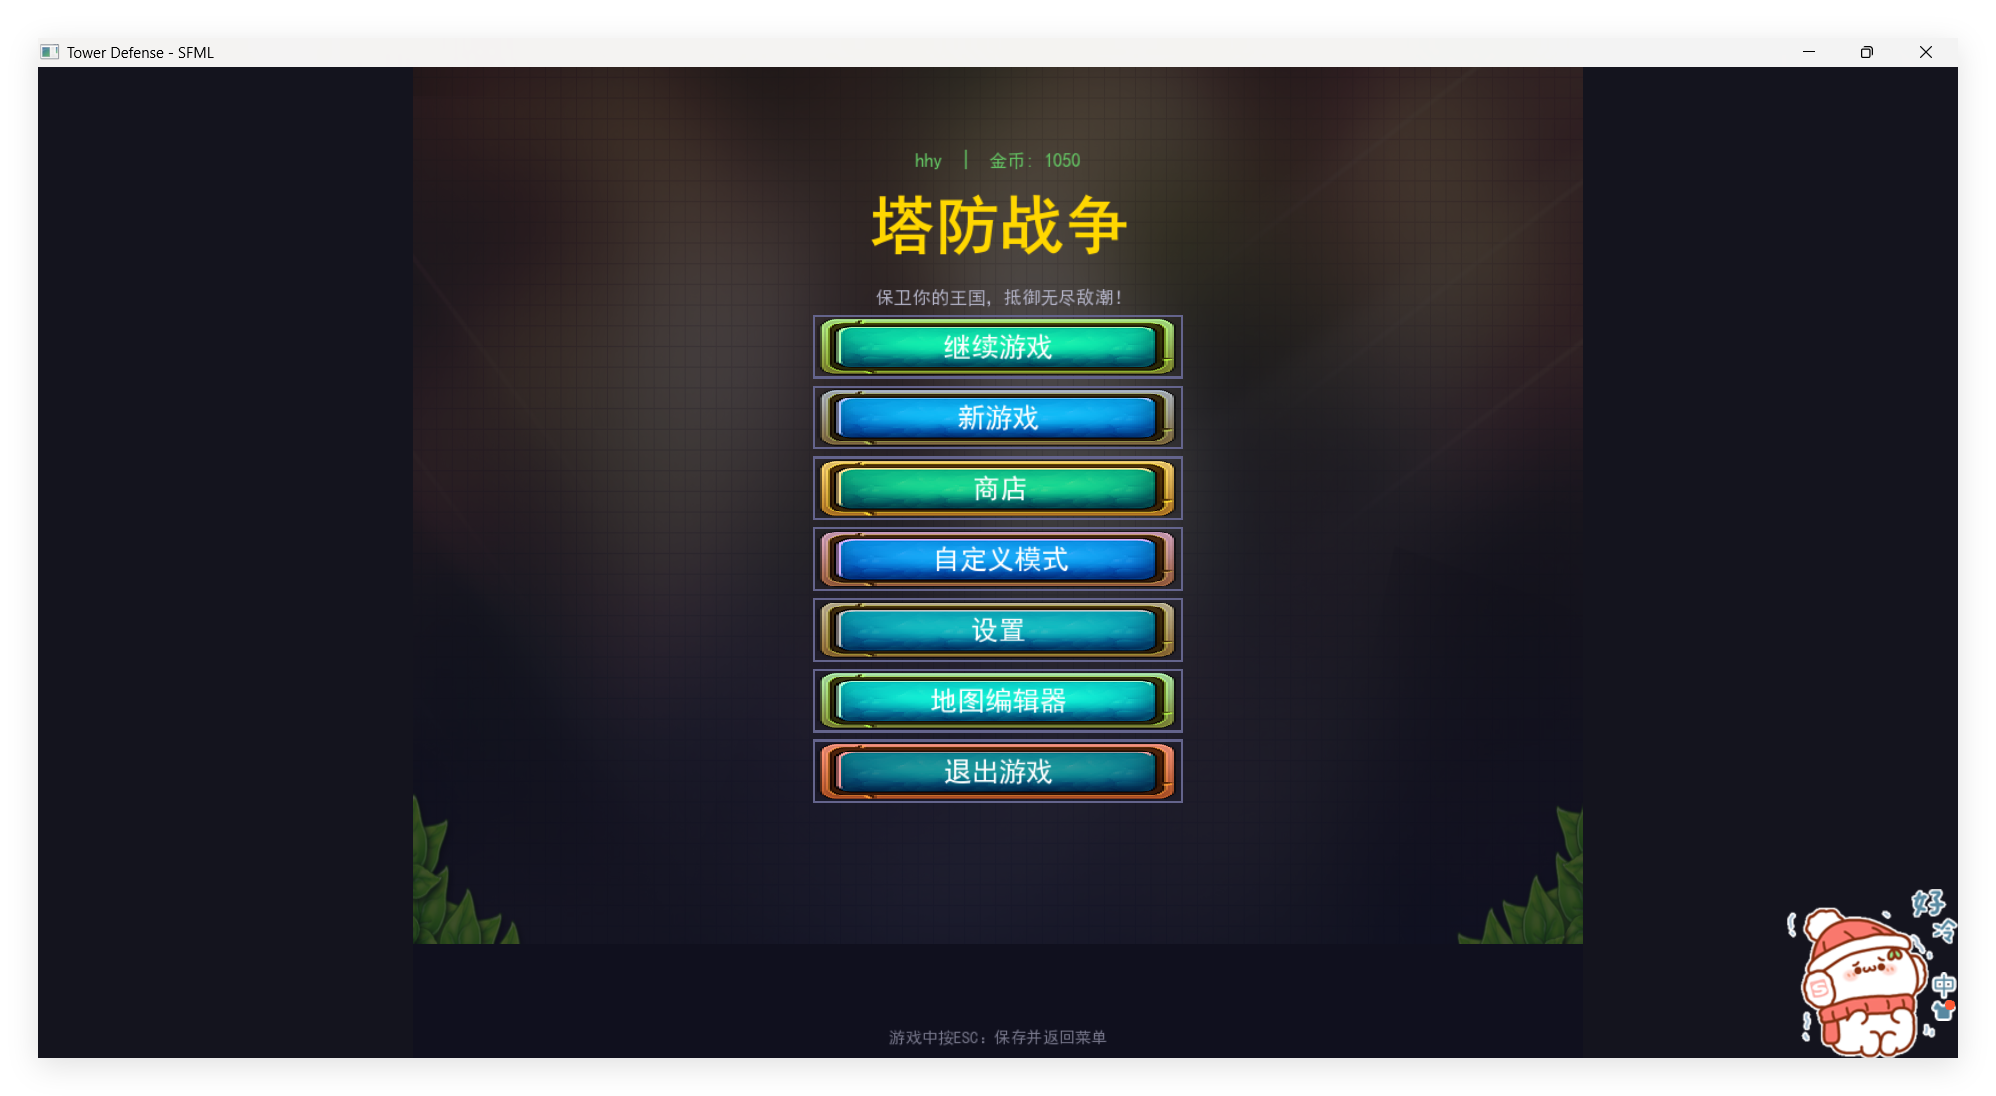
\includegraphics[width=\textwidth]{menu.png}
    \caption{中文界面——主菜单}
    \end{subfigure}
    \hfill  % 在两个子图之间插入水平空白，让它们分开
    \begin{subfigure}[b]{0.45\textwidth}
        \centering
        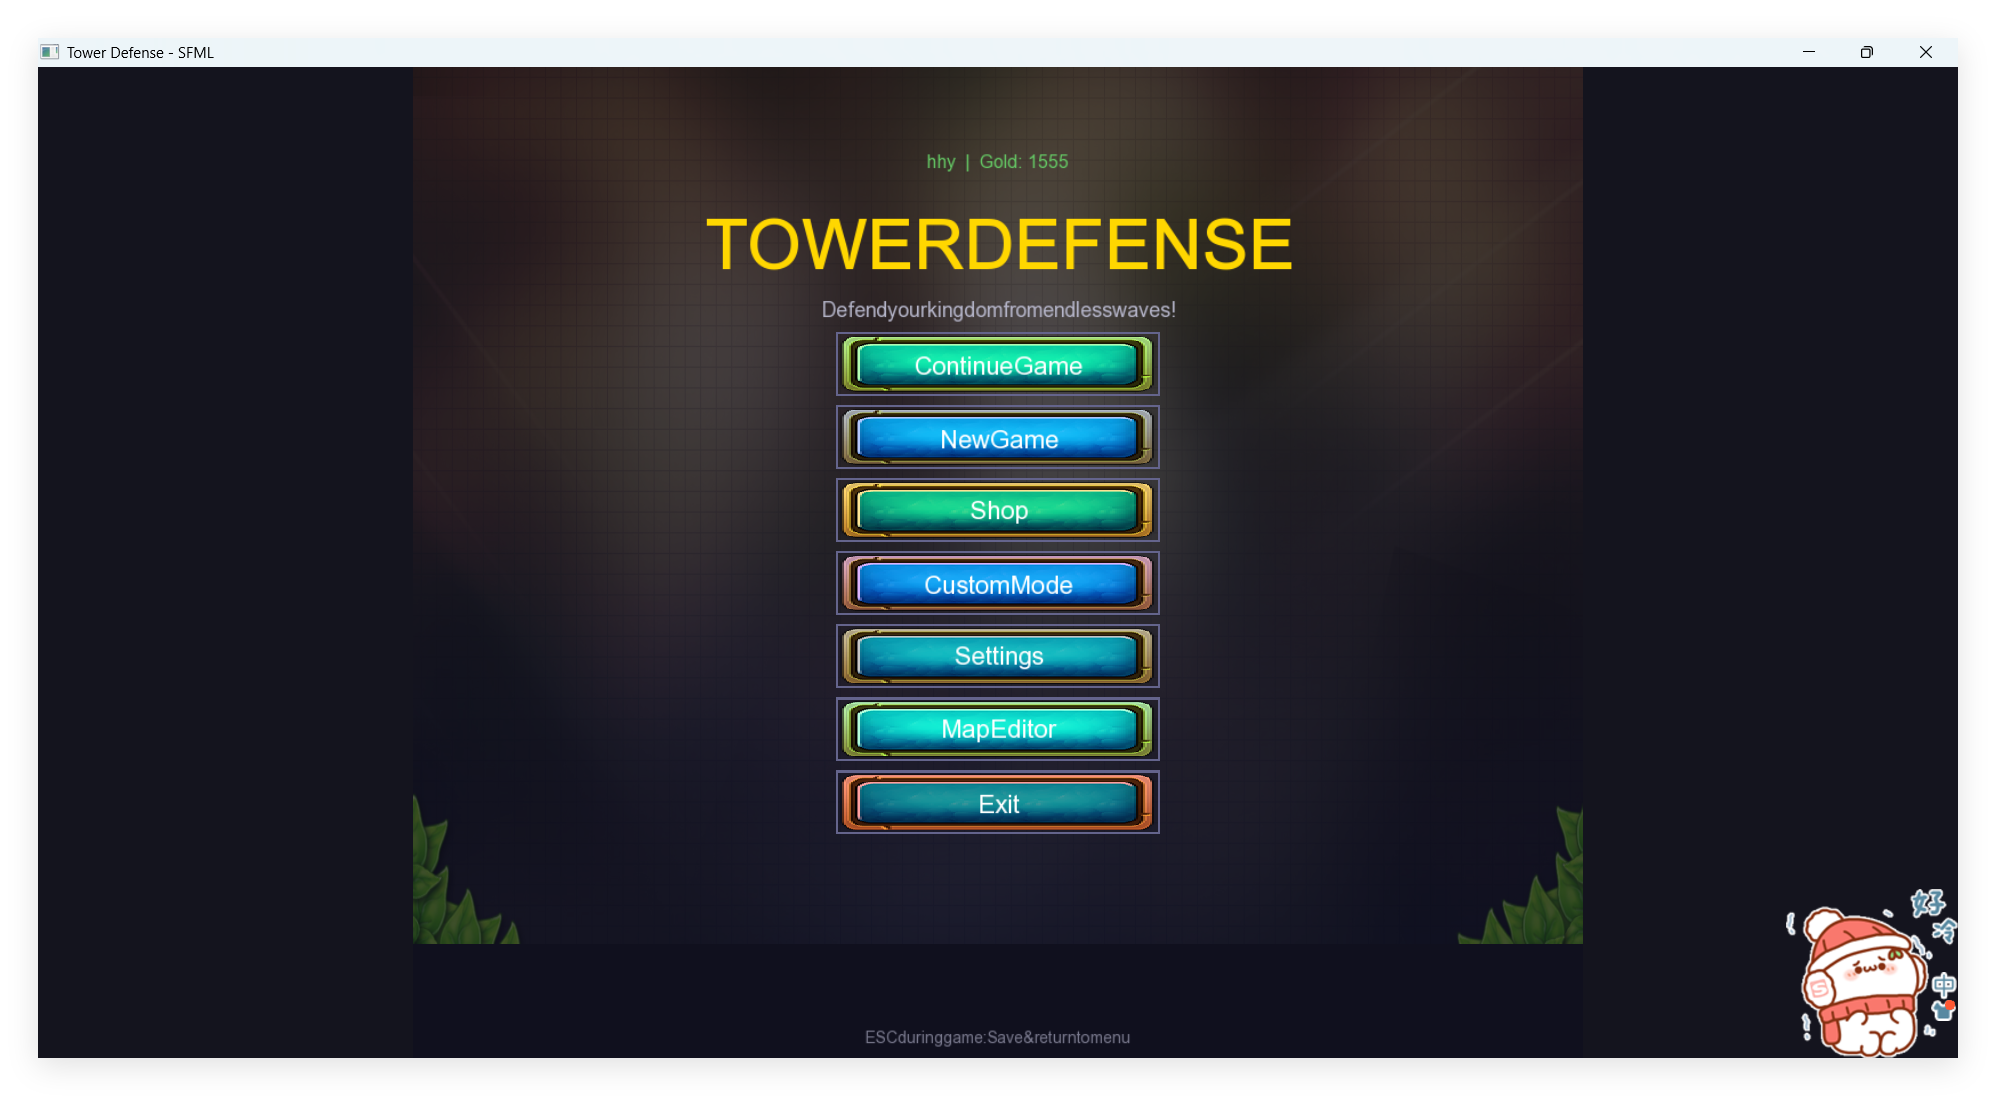
\includegraphics[width=\textwidth]{menu_en.png}
        \caption{英文界面——主菜单}
    \end{subfigure}
    \caption{主菜单}  % 可选：整个 figure 的大标题
\end{figure}

\section{作弊码系统}

灵感来自《罪恶都市》的键盘输入作弊码，游戏进行中直接输入：

\begin{table}[H]
    \centering
    \caption{作弊码列表}
    \begin{tabularx}{\textwidth}{lX}
        \toprule
        \textbf{作弊码} & \textbf{效果} \\
        \midrule
        money     & 无限金币 \\
        morepower & 无限伤害（一击必杀） \\
        killall   & 秒杀所有当前敌人 \\
        winlevel  & 立即通关当前关卡 \\
        boss      & 生成一只 Boss \\
        unlockall & 临时解锁所有关卡 \\
        lastwave  & 直接跳到最后一波 \\
        \bottomrule
    \end{tabularx}
\end{table}

\begin{lstlisting}[caption={Game::processCheatInput()——环形缓冲区匹配}]
void Game::processCheatInput(sf::Uint32 unicode)
{
    // 自动转小写，追加到环形缓冲区
    if (unicode >= 'A' && unicode <= 'Z')
        unicode += ('a' - 'A');
    if (unicode < 'a' || unicode > 'z')
        return;
    m_cheatBuffer[m_cheatBufLen++] = (char)unicode;
    m_cheatBuffer[m_cheatBufLen] = '\0';

    // 缓冲区中搜索匹配的作弊码
    std::string buf(m_cheatBuffer);
    if (buf.find("money") != std::string::npos)
        activateCheat("money");
    else if (buf.find("killall") != std::string::npos)
        activateCheat("killall");
    // ... 其余作弊码同理
}

void Game::activateCheat(const std::string &code)
{
    clearCheatBuffer();
    // 切换开关或执行即时效果
    if (code == "money")  m_infiniteGold = !m_infiniteGold;
    if (code == "killall") killAllEnemies();
    // 显示金色大字提示，3秒后自动消失
    m_cheatMsgText.setFillColor(sf::Color(255, 215, 0));
    m_cheatMsgClock.restart();
}
\end{lstlisting}

作弊码通过 \texttt{sf::Event::TextEntered} 捕获键盘输入，存储在环形缓冲区中匹配。

\begin{figure}[H]
    \centering
    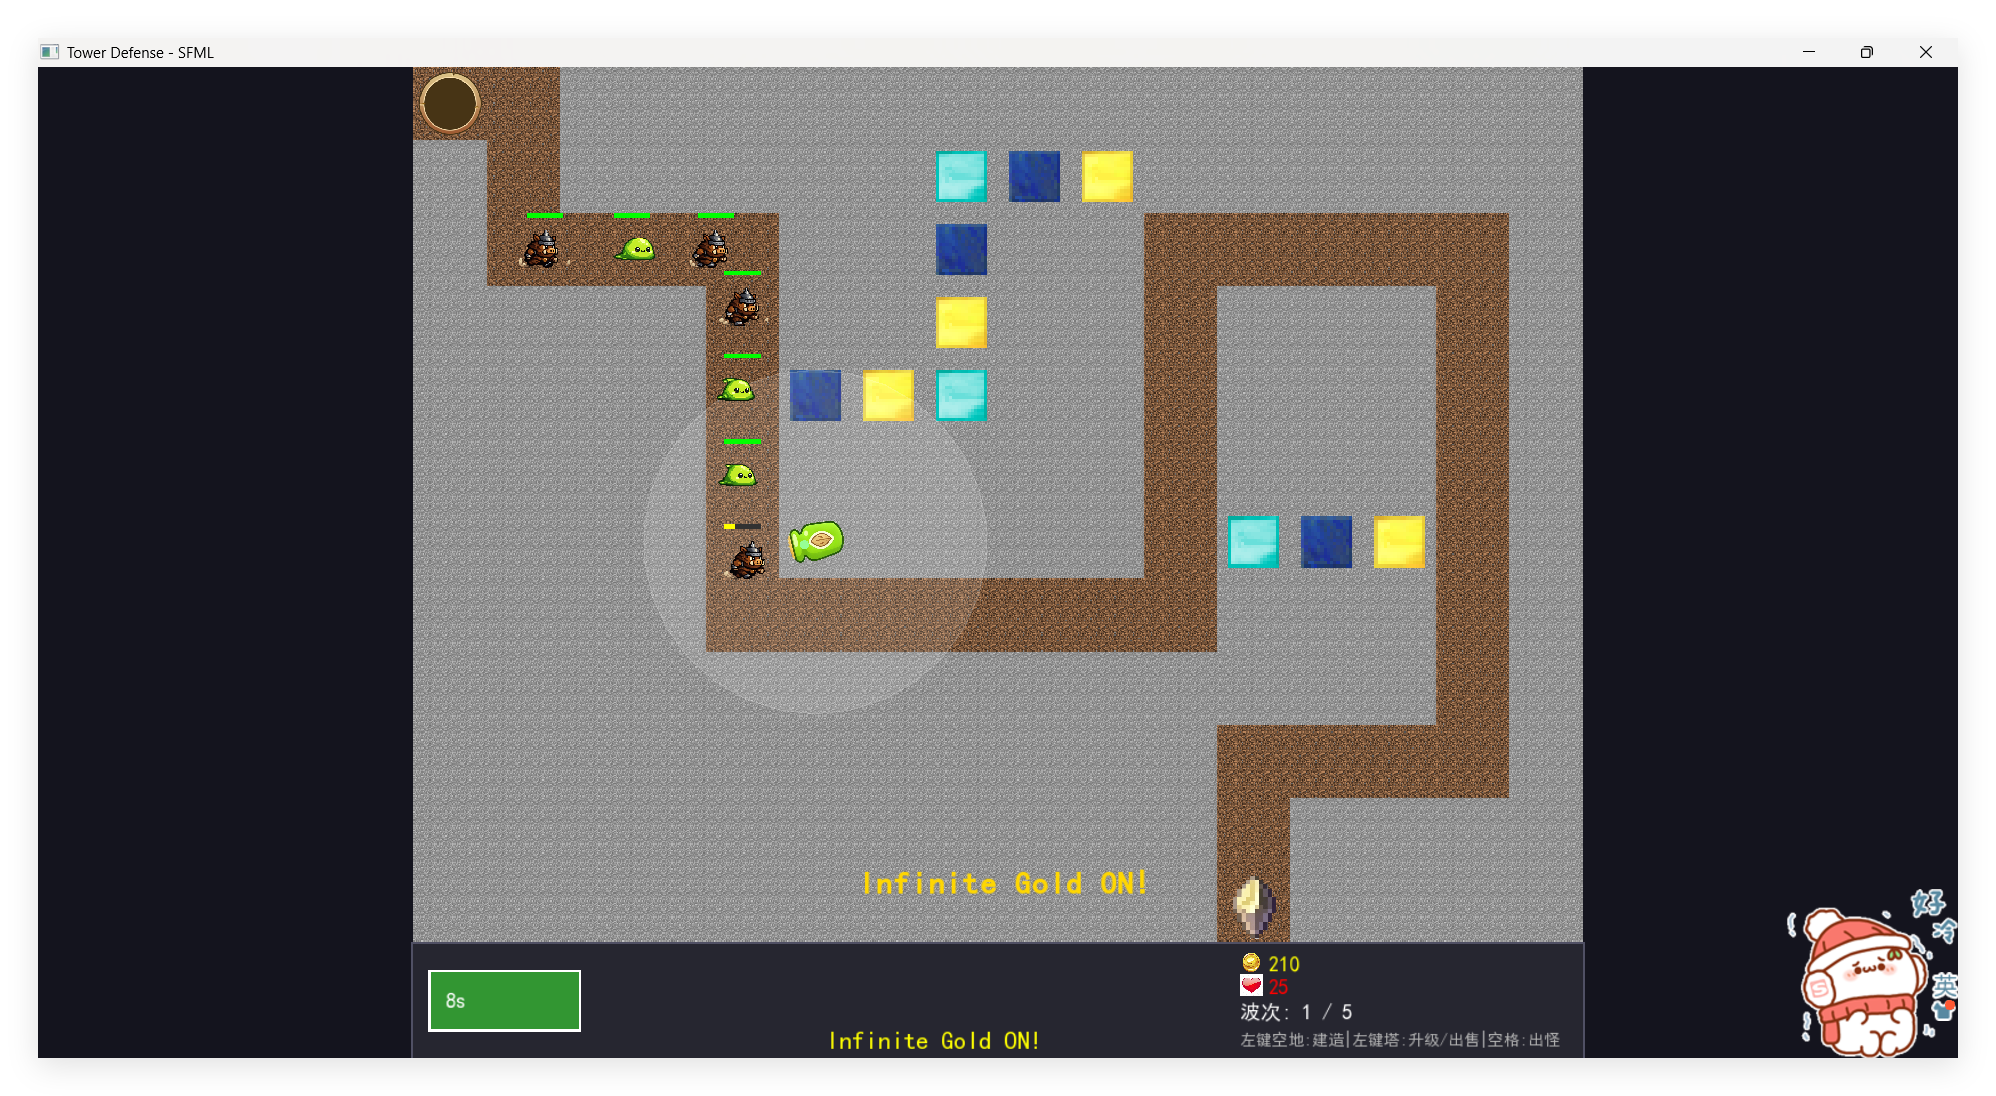
\includegraphics[width=0.7\textwidth]{cheat1.png}
    \caption{作弊码效果展示}
\end{figure}


\section{地图编辑器}

\subsection{功能}

\begin{itemize}
    \item 在游戏内直接编辑地图
    \item 通过数字键 0-4 切换瓦片类型
    \item 编辑网格 16×12
    \item 支持保存地图到文件
    \item 支持在地图编辑器中命名文件
\end{itemize}

\subsection{操作}

\begin{itemize}
    \item 左键点击放置当前选中的瓦片
    \item 数字键切换编辑模式
    \item 保存时输入文件名
\end{itemize}


\section{场景、人物与动画的创建}

\subsection{场景创建}

游戏场景基于瓦片地图（Tile Map）系统构建，每个瓦片 64×64 像素，形成 16×12 的网格。

\textbf{地图数据格式}：地图文件为纯文本，每行 16 个整数，共 12 行。数字 0=草地、1=路径、2=出生点、3=终点、4=障碍。路径查找器（C 语言实现）从起点出发沿路径追踪到终点，生成路点序列供敌人跟随。

\textbf{群系纹理}：游戏支持 4 种群系（Grassland / Desert / Hell / Community），每种群系有独立的地面纹理（ground1-3.png）和装饰纹理（kong1-3.png）。通过 \texttt{Map::loadBiomeTextures()} 动态切换。

\textbf{渲染流程}：每帧 \texttt{Map::draw()} 遍历 16×12 网格，根据瓦片类型绘制对应的精灵。草地绘制装饰纹理，路径绘制地面纹理，起点/终点叠加标记精灵，障碍物上可能叠放宝藏精灵。整个场景使用 SFML 的 \texttt{sf::Sprite} 渲染，纹理通过 \texttt{sf::Texture::loadFromFile()} 加载。

\textbf{宝藏渲染}：三种宝藏纹理（Treasure1-3.png）随机分配到障碍物上，被攻击后 3 秒内显示血条（\texttt{sf::RectangleShape}），血条颜色随剩余血量变化（绿→黄→红）。

\subsection{人物创建}

游戏中的人物分为塔和敌人两类：

\textbf{塔的纹理}：三种塔各有 3 级外观，共 9 个独立 PNG 文件（Arrow\_level1-3.png、Cannon\_level1-3.png、Ice\_level1-3.png）。每座塔通过 \texttt{Tower::loadTextures()} 静态加载所有纹理到 \texttt{static sf::Texture s\_textures[3][3]} 数组，所有塔实例共享同一份纹理，避免重复加载。

塔的炮口旋转使用 \texttt{m\_sprite.setRotation(m\_targetAngle)}，角度由 \texttt{std::atan2()} 根据目标方向计算（冰塔不旋转）。

\textbf{敌人的纹理与动画}：敌人使用精灵表（Sprite Sheet）实现帧动画。每个纹理文件横向包含 4 帧（如 enemy1.png 宽度为 4 帧之和）。

\begin{figure}[H]
    \centering
    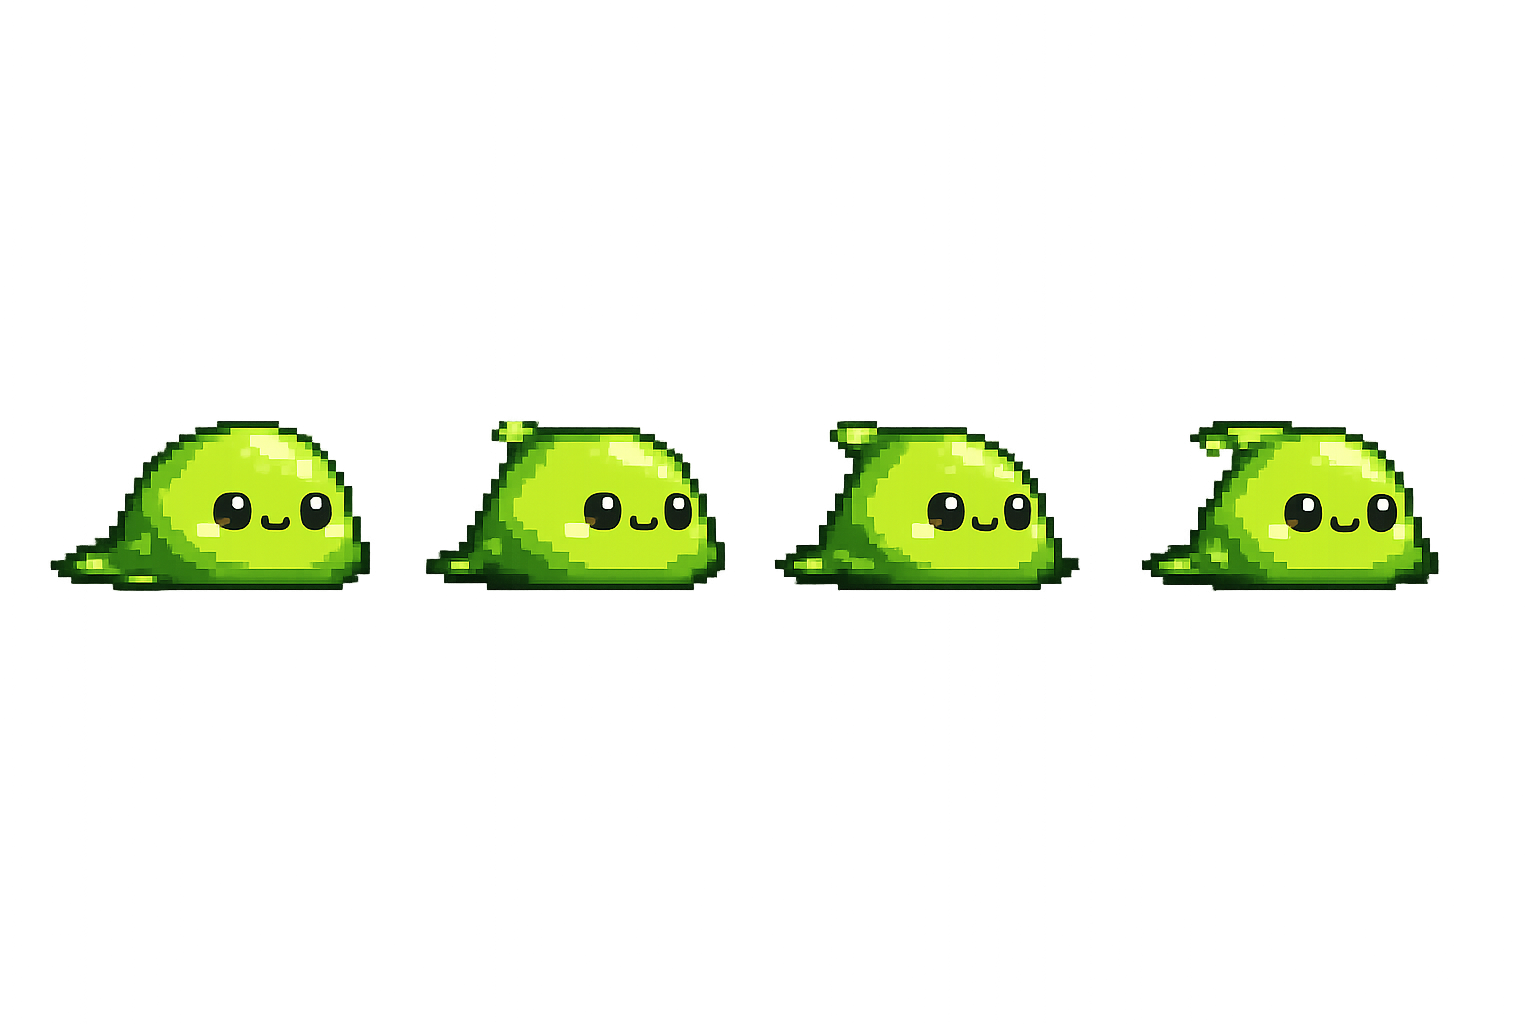
\includegraphics[width=0.5\textwidth]{../textures/enemy1.png}
    \caption{enemy1.png——绿色史莱姆精灵表，横向4帧行走动画}
\end{figure}

动画实现如下：

\begin{lstlisting}[caption={敌人4帧动画实现}]
// 纹理水平切分为4帧
auto sz = s_textures[m_variant].getSize();
int frameWidth = sz.x / 4;

// 每帧更新动画帧（0.15秒切换一帧）
m_animTimer += dt;
if (m_animTimer >= 0.15f) {
    m_animTimer = 0;
    m_animFrame = (m_animFrame + 1) % 4;
}

// 设置纹理矩形区域为当前帧
m_sprite.setTextureRect(
    sf::IntRect(m_animFrame * frameWidth, 0,
                frameWidth, sz.y));
\end{lstlisting}

\textbf{Boss 纹理}：两种 Boss（boss1.png、boss2.png）拥有独立的纹理和更高倍率的属性，在最后一波以特殊方式生成。

\subsection{弹丸与特效}

弹丸使用 SFML 的几何图形 \texttt{sf::CircleShape} 而非纹理，通过颜色区分类型：
\begin{itemize}
    \item 箭弹：绿色圆形
    \item 炮弹：红色圆形
    \item 冰弹：蓝色圆形
\end{itemize}

弹丸沿直线飞向目标，击中后标记销毁。冰弹击中敌人时触发减速特效（\texttt{applySlow()} 将敌人速度降至 40\%，持续 2 秒）。

\subsection{纹理与资源制作}

\begin{itemize}
    \item \textbf{纹理格式}：所有游戏纹理使用 PNG 格式，支持透明通道
    \item \textbf{尺寸规格}：塔纹理和敌人纹理按瓦片大小（64×64）的适配比例设计
    \item \textbf{制作工具}：纹理使用图像编辑软件（如 Photoshop、GIMP）绘制
    \item \textbf{动画制作}：敌人动画帧水平排列在同一 PNG 中，通过 \texttt{sf::IntRect} 裁切获取当前帧
    \item \textbf{字体}：英文使用 Arial，中文使用 SimHei（黑体），均为 TTF 格式
    \item \textbf{音频}：背景音乐为 MP3 格式，通过 \texttt{sf::Music} 流式播放
\end{itemize}


\section{技术细节}

\subsection{主循环}

\begin{lstlisting}[caption={Game::run() 主循环伪代码}]
while (window.isOpen())
    processEvents()       // 处理所有输入事件
    update(dt)            // 更新游戏状态
    render()              // 渲染当前帧
    window.display()      // 交换缓冲区
\end{lstlisting}

\subsection{弹丸系统}

\begin{itemize}
    \item \texttt{Projectile} 类支持两种构造方式：
    \begin{enumerate}
        \item 追踪敌人：持有 \texttt{weak\_ptr<Enemy>} 目标引用
        \item 固定位置：用于宝藏攻击
    \end{enumerate}
    \item 弹丸击中后标记 \texttt{m\_hasHit = true}
    \item 通过 \texttt{checkProjectileCollisions()} 处理碰撞效果
\end{itemize}

\subsection{性能设计}

\begin{itemize}
    \item 使用 \texttt{std::vector<std::shared\_ptr<T>>} 管理动态对象
    \item 使用 \texttt{std::weak\_ptr} 避免弹丸和塔之间的循环引用
    \item 使用 \texttt{std::remove\_if + erase} 惯用语法移除死亡对象
    \item 瓦片网格固定大小 16×12，使用栈上数组避免动态分配
    \item 纹理静态加载，所有实例共享同一份纹理
\end{itemize}

\subsection{存档格式}

角色存档为二进制文件，包含：
\begin{itemize}
    \item 角色名（字符串）
    \item 累计金币（int）
    \item 已解锁关卡数（int）
    \item 6 个商店项目等级（int 数组）
\end{itemize}

\begin{lstlisting}[caption={PlayerData 存档结构}]
struct PlayerData {
    std::string name;
    int totalGold;
    int unlockedLevels;
    int shopLevels[6];  // ShopItem 的 COUNT
};
\end{lstlisting}

\subsection{资源目录}

\begin{lstlisting}
assets/
├── lang_en.json       # 英文语言包
├── lang_zh.json       # 中文语言包
└── maps/
    ├── grassland/     # 1-1.txt, 1-2.txt, 1-3.txt
    ├── desert/        # 2-1.txt, 2-2.txt, 2-3.txt
    ├── hell/          # 3-1.txt, 3-2.txt, 3-3.txt
    └── community/     # c1.txt, c2.txt, custom_editor.txt

textures/
├── Arrow_level[1-3].png     # 箭塔 3 级纹理
├── Cannon_level[1-3].png    # 炮塔 3 级纹理
├── Ice_level[1-3].png       # 冰塔 3 级纹理
├── enemy[1-3].png            # 敌人纹理（4 帧动画）
├── boss[1-2].png             # Boss 纹理
├── Treasure[1-3].png         # 宝藏纹理
├── ground[1-3].png           # 地面纹理（群系）
├── kong[1-3].png             # 空地纹理（群系）
├── birth.png                 # 出生点标记
├── endpoint.png              # 终点标记
├── gold.png / life.jpg       # UI 图标
├── Button*.png               # UI 按钮
├── Arrowleft/Arrowright.png  # 箭头按钮
└── information.png           # 信息图标

fonts/
├── arial.ttf                 # 英文字体
└── simhei.ttf                # 中文字体

sound/
└── bgm.mp3                   # 背景音乐
\end{lstlisting}


\section{游戏流程示例}

以战役模式 1-1 为例：

\begin{enumerate}
    \item 玩家创建角色 → 进入主菜单
    \item 点击"新游戏" → 进入战役选择
    \item 选择 1-1（Green Meadow）
    \item 游戏初始化：
    \begin{itemize}
        \item 加载地图 \texttt{assets/maps/grassland/1-1.txt}
        \item 金币 250，生命 25，5 波敌人
        \item 速度 0.9 倍，HP 0.8 倍
        \item 应用角色商店加成
    \end{itemize}
    \item 玩家在 Grass 格子上点击 → 建造弹窗 → 选择塔
    \item 10 秒倒计时或点击"Start Wave" → 开始出怪
    \item 敌人沿路径前进 → 塔自动攻击 → 获得金币
    \item 手动开始后续波次获得额外金币奖励
    \item 波次 5（最后一波）可能出现 Boss
    \item 全波次完成 → 胜利界面 → 累计金币 → 解锁 1-2
\end{enumerate}

\begin{figure}[H]
    \centering
    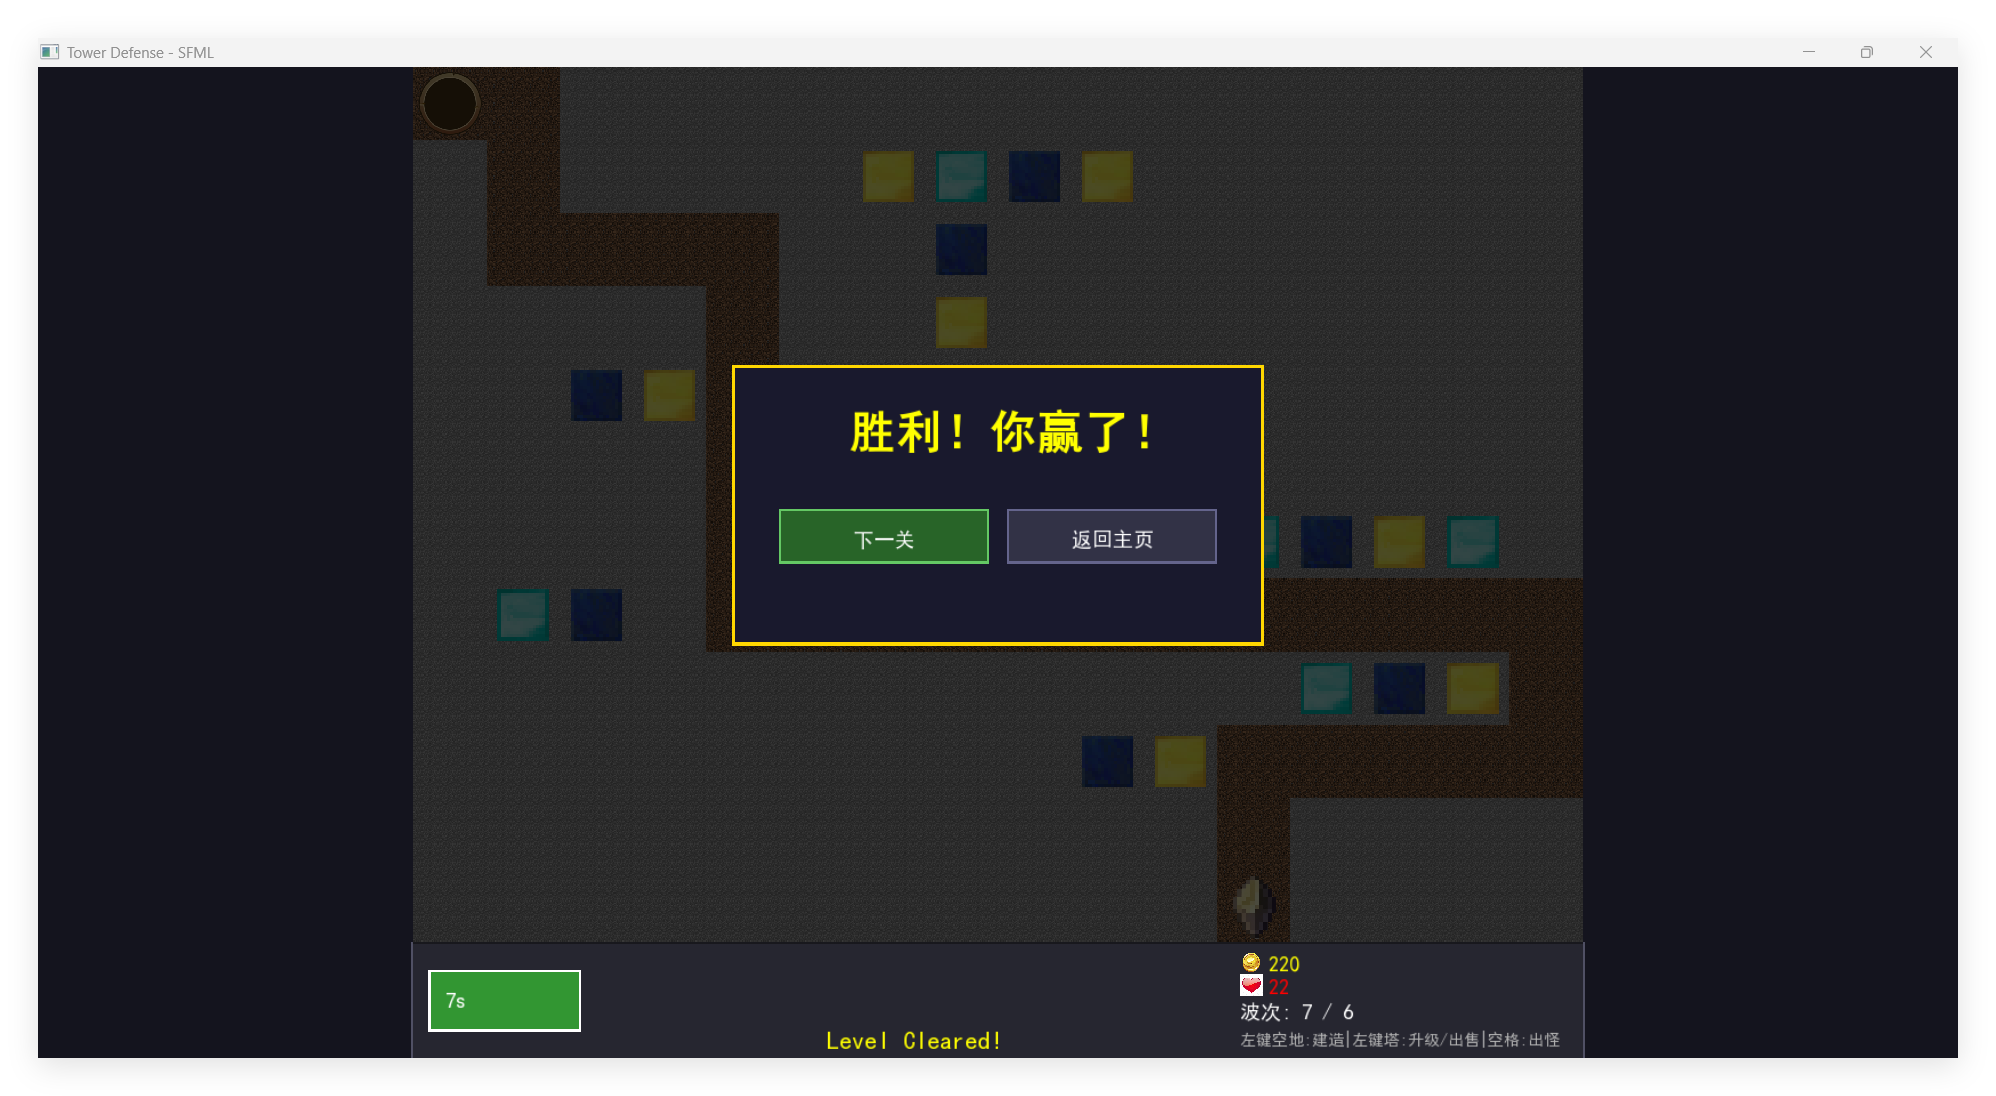
\includegraphics[width=0.7\textwidth]{victory.png}
    \caption{通关胜利界面}
\end{figure}

\begin{figure}[H]
    \centering
    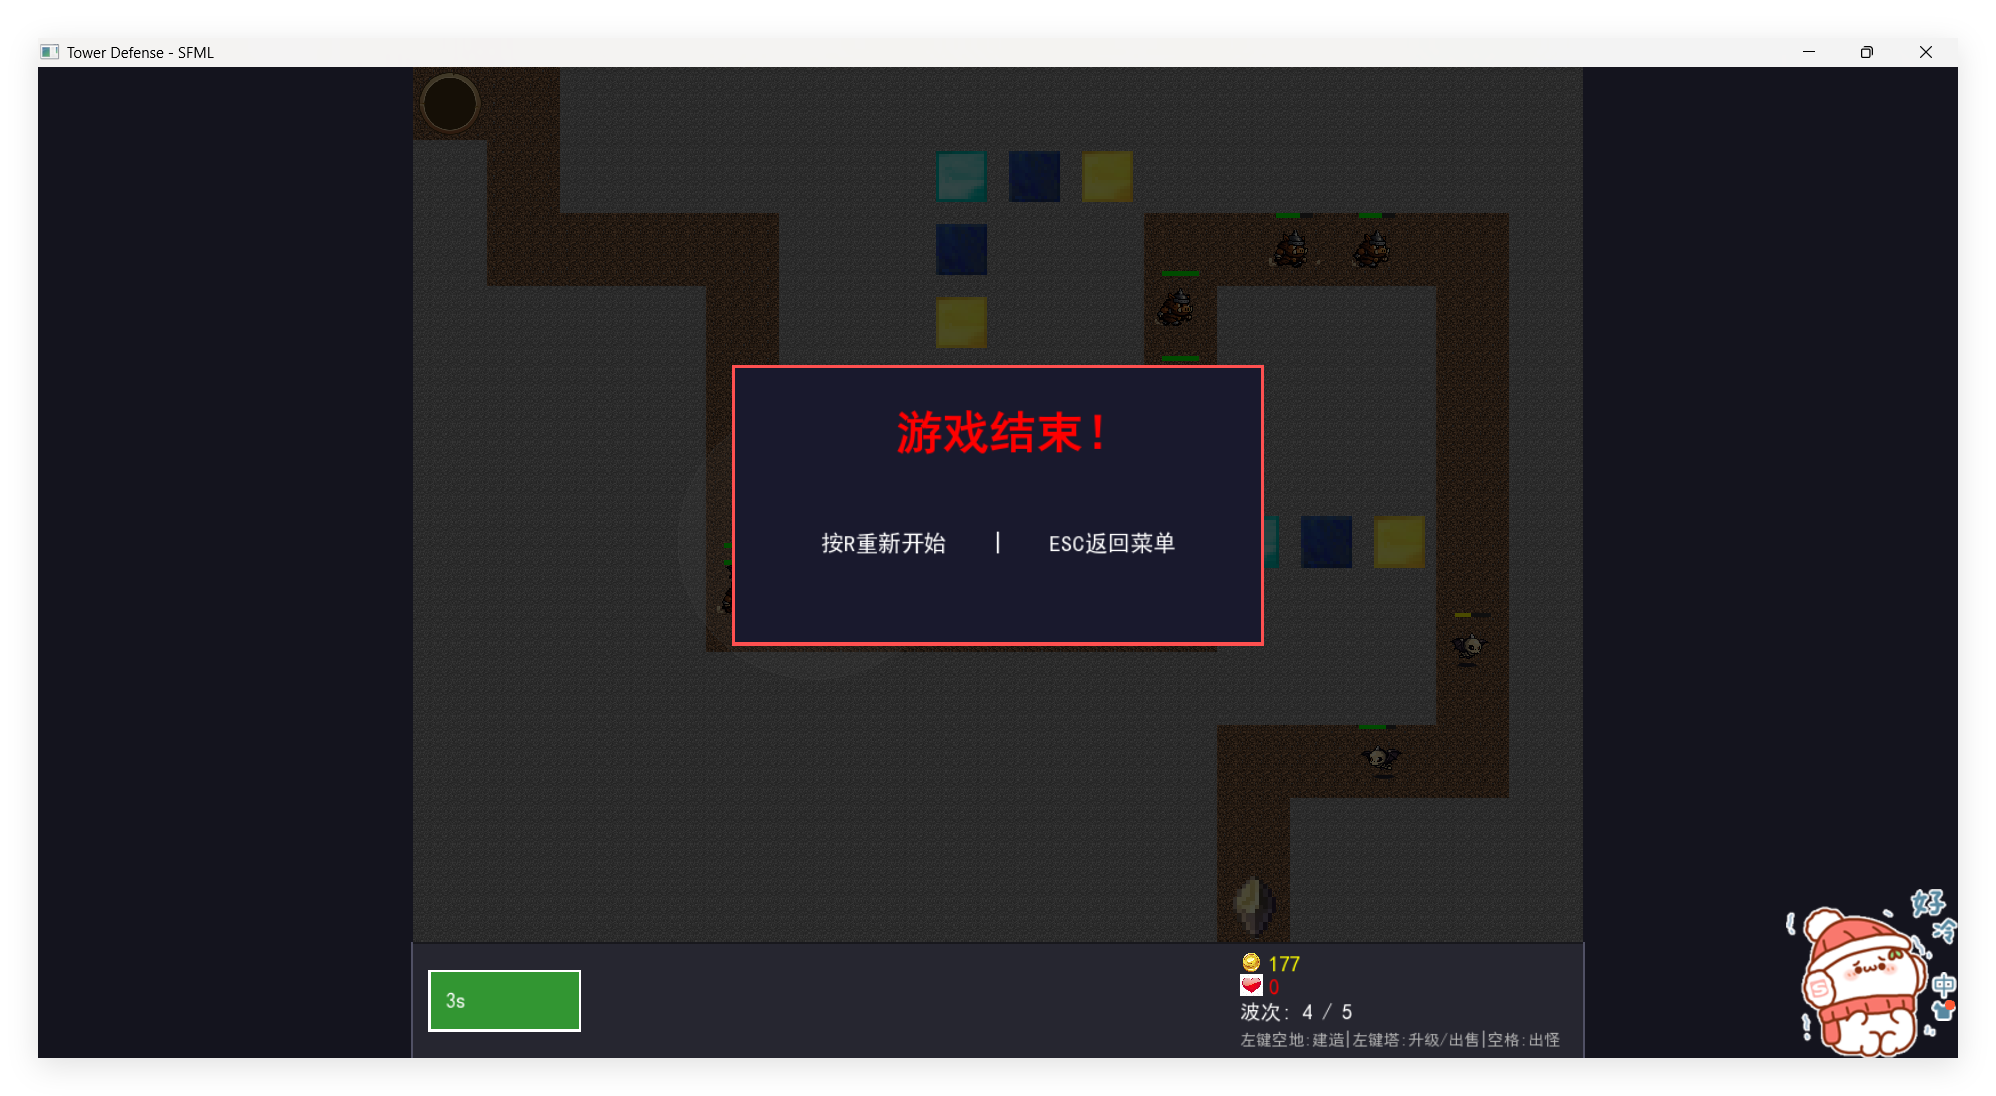
\includegraphics[width=0.7\textwidth]{game_over.png}
    \caption{游戏失败界面}
\end{figure}


\section{游戏玩法说明}

\subsection{游戏目标}

在每一关中，玩家需要在敌人抵达终点前将其全部消灭。每有一个敌人到达终点则扣除一条生命，生命归零则游戏失败。成功抵御所有波次即为通关。

\subsection{基本操作}

\begin{table}[H]
    \centering
    \caption{游戏操作说明}
    \begin{tabularx}{\textwidth}{lX}
        \toprule
        \textbf{操作} & \textbf{说明} \\
        \midrule
        左键点击空地 & 打开建造弹窗，选择塔类型建造 \\
        左键点击已有塔 & 打开塔管理弹窗，选择升级或出售 \\
        左键点击宝藏 & 命令塔集中攻击该宝藏 \\
        右键 & 关闭弹出菜单 \\
        空格键 & 手动开始下一波敌人 \\
        Esc & 暂停游戏，可选择继续或保存返回主菜单 \\
        R（失败时） & 重新开始当前关卡 \\
        \bottomrule
    \end{tabularx}
\end{table}

\subsection{新手入门}

\begin{enumerate}
    \item \textbf{创建角色}：首次运行游戏时，输入角色名并创建存档
    \item \textbf{选择模式}：主菜单中点击"新游戏"进入战役，或选择"自定义模式"自由设置参数
    \item \textbf{建造防御}：在草地上点击左键，选择箭塔或炮塔建造（冰塔辅助减速）
    \item \textbf{开始战斗}：等待倒计时或按空格键/点击"Start Wave"开始出怪
    \item \textbf{经营资源}：击杀敌人获得金币，用于建造更多塔或升级现有塔
    \item \textbf{挑战Boss}：最后一波可能出现 Boss，提前积累火力
\end{enumerate}

\subsection{策略建议}

\begin{itemize}
    \item \textbf{混合布塔}：箭塔均衡输出、炮塔高伤害、冰塔减速控场，三者配合效果最佳
    \item \textbf{集中升级}：将资源优先升级 1-2 座核心塔比分散建造低级塔更有效
    \item \textbf{弯道布置}：在路径拐弯处集中布塔，延长敌人通过火力区的时间
    \item \textbf{手动开波}：手动开始波次可获得额外金币奖励，积少成多
    \item \textbf{攻击宝藏}：打碎宝藏可获得大量金币，是快速发育的重要途径
    \item \textbf{商店投资}：跨关卡金币用于商店升级，优先提升伤害和起始金币
\end{itemize}


\section{与同类游戏的比较与创新}

\subsection{同类游戏对比}

本游戏在玩法上借鉴了经典塔防游戏的设计理念，同时在多个方面做出了差异化：

\begin{table}[H]
    \centering
    \caption{与同类塔防游戏的特性对比}
    \begin{tabularx}{\textwidth}{lXXX}
        \toprule
        \textbf{特性} & \textbf{本游戏} & \textbf{同类塔防} \\
        \midrule
        塔类型 & 箭塔/炮塔/冰塔（3种） & 通常 4-8 种 \\
        塔升级 & 3级，线性增长 & 通常 2-4 级 \\
        地图 & 固定路径瓦片地图 & 固定路径或自由摆放 \\
        出怪方式 & 自动倒计时 + 手动触发 & 通常自动连续 \\
        敌人系统 & 加权随机变体 + Boss & 固定波次配置 \\
        跨关卡成长 & 角色+商店6项升级 & 稀有或需DLC \\
        多语言 & 中英文动态切换 & 通常仅单语言 \\
        内置编辑器 & 完整地图编辑器 & 少数支持 \\
        作弊码 & 隐形键盘输入（罪恶都市风格） & 通常为控制台指令 \\
        \bottomrule
    \end{tabularx}
\end{table}

\subsection{创新玩法}

\subsubsection{宝藏攻坚系统}

地图上散布着可破坏的宝藏方块，每块拥有独立血量（3/5/8 HP）。玩家点击宝藏即可命令所有射程内的塔集火攻击。宝藏被击破后返还 50/100/150 金币，并将该格子变为可建造区域。这一机制在传统塔防"建塔→打怪"的循环中增加了地图探索和目标选择的策略维度。

\subsubsection{罪恶都市风格作弊码}

与传统游戏使用控制台或菜单开关作弊不同，本游戏实现了类似《侠盗猎车手：罪恶都市》的隐形键盘输入系统。玩家在游戏过程中直接依次按下键盘字母，系统在环形缓冲区中实时匹配预定义作弊码字符串。匹配成功后通过全屏金色大字显示反馈，增强了趣味性和复古游戏体验。

\subsubsection{内置地图编辑器}

游戏自带完整的地图编辑器，玩家无需借助外部工具即可创建和编辑关卡。编辑器支持：
\begin{itemize}
    \item 数字键 0-4 切换瓦片类型
    \item 左键点击放置瓦片
    \item 自定义文件名保存
    \item 保存后的地图可在自定义模式中选用
\end{itemize}

\subsubsection{跨关卡角色成长体系}

通过引入 RPG 风格的"角色"概念，玩家的游戏进度、累计金币、商店升级等级被持久化保存，形成跨关卡的成长循环。6 种商店升级（起始金币、塔折扣、伤害、射程、生命、攻速）让玩家在多次游玩中逐渐积累优势，增加了游戏的长期可玩性和回放价值。

\subsubsection{自定义模式}

玩家可自由调整波次数量、每波敌人数、起始金币、起始生命、速度倍率、HP 倍率和地图，创造出从"休闲体验"到"地狱难度"的任意游戏体验，大幅拓展了游戏的生命周期。

\subsection{改进方向}

\begin{itemize}
    \item \textbf{更多塔类型}：引入魔法塔、毒塔、狙击塔等差异化塔种
    \item \textbf{技能系统}：玩家可使用全屏技能（轰炸、冰冻、金币雨）
    \item \textbf{联网对战}：支持双人合作或 PvP 竞技模式
    \item \textbf{成就系统}：完成特定挑战解锁成就和奖励
    \item \textbf{地图工坊}：支持社区地图分享与评分
    \item \textbf{移动端适配}：触控交互优化与性能调优
\end{itemize}


\section{总结}

本游戏实现了经典塔防的核心玩法，并在此基础上扩展了丰富的周边系统：

\begin{itemize}
    \item \textbf{三种特色塔类型}：箭塔均衡输出、炮塔高伤害、冰塔减速控场，提供策略多样性
    \item \textbf{三级升级系统}：每级 60\% 伤害增幅，鼓励集中资源升级核心塔
    \item \textbf{多群系战役关卡}：草地/沙漠/地狱三大群系渐进式难度曲线
    \item \textbf{宝藏攻坚系统}：可破坏的障碍物，集火攻击获得额外金币和建造空间
    \item \textbf{罪恶都市作弊码}：隐形键盘输入，金色大字反馈，增加趣味性
    \item \textbf{内置地图编辑器}：无需外部工具即可创建和编辑关卡
    \item \textbf{跨关卡角色成长}：RPG风格的角色存档与6项商店升级
    \item \textbf{双模式并存}：固定战役 + 完全可自定义的自由模式
    \item \textbf{多语言支持}：中英文运行时动态切换
\end{itemize}

\textbf{场景创建}方面，游戏采用瓦片地图系统，通过 16×12 网格和 4 种群系纹理构建多样化的视觉场景。\textbf{人物与动画}方面，三种塔使用独立的等级纹理，敌人通过精灵表实现 4 帧行走动画，弹丸使用 SFML 几何图形渲染。\textbf{交互设计}方面实现了弹出菜单、HUD 信息反馈、暂停菜单、确认对话框等完整的交互体系。

与同类塔防游戏相比，本游戏在宝藏集火机制、隐形作弊码输入、内置地图编辑器、跨关卡角色成长等方面做出了差异化创新。整个项目基于 SFML 2.6 引擎使用 C++17 实现，代码结构清晰（约 25 个源文件），从底层图形渲染到上层游戏逻辑均有完整实现，是一个具备参考价值的塔防游戏工程实践。

\end{document}
